% Options for packages loaded elsewhere
\PassOptionsToPackage{unicode}{hyperref}
\PassOptionsToPackage{hyphens}{url}
%
\documentclass[
]{article}
\usepackage{lmodern}
\usepackage{amssymb,amsmath}
\usepackage{ifxetex,ifluatex}
\ifnum 0\ifxetex 1\fi\ifluatex 1\fi=0 % if pdftex
  \usepackage[T1]{fontenc}
  \usepackage[utf8]{inputenc}
  \usepackage{textcomp} % provide euro and other symbols
\else % if luatex or xetex
  \usepackage{unicode-math}
  \defaultfontfeatures{Scale=MatchLowercase}
  \defaultfontfeatures[\rmfamily]{Ligatures=TeX,Scale=1}
\fi
% Use upquote if available, for straight quotes in verbatim environments
\IfFileExists{upquote.sty}{\usepackage{upquote}}{}
\IfFileExists{microtype.sty}{% use microtype if available
  \usepackage[]{microtype}
  \UseMicrotypeSet[protrusion]{basicmath} % disable protrusion for tt fonts
}{}
\makeatletter
\@ifundefined{KOMAClassName}{% if non-KOMA class
  \IfFileExists{parskip.sty}{%
    \usepackage{parskip}
  }{% else
    \setlength{\parindent}{0pt}
    \setlength{\parskip}{6pt plus 2pt minus 1pt}}
}{% if KOMA class
  \KOMAoptions{parskip=half}}
\makeatother
\usepackage{xcolor}
\IfFileExists{xurl.sty}{\usepackage{xurl}}{} % add URL line breaks if available
\IfFileExists{bookmark.sty}{\usepackage{bookmark}}{\usepackage{hyperref}}
\hypersetup{
  pdftitle={Nudging for less kludges: focusing on PMD alerts as possible kludges: open, fixed or new?},
  pdfauthor={Bruno Crotman},
  hidelinks,
  pdfcreator={LaTeX via pandoc}}
\urlstyle{same} % disable monospaced font for URLs
\usepackage[margin=1in]{geometry}
\usepackage{color}
\usepackage{fancyvrb}
\newcommand{\VerbBar}{|}
\newcommand{\VERB}{\Verb[commandchars=\\\{\}]}
\DefineVerbatimEnvironment{Highlighting}{Verbatim}{commandchars=\\\{\}}
% Add ',fontsize=\small' for more characters per line
\usepackage{framed}
\definecolor{shadecolor}{RGB}{248,248,248}
\newenvironment{Shaded}{\begin{snugshade}}{\end{snugshade}}
\newcommand{\AlertTok}[1]{\textcolor[rgb]{0.94,0.16,0.16}{#1}}
\newcommand{\AnnotationTok}[1]{\textcolor[rgb]{0.56,0.35,0.01}{\textbf{\textit{#1}}}}
\newcommand{\AttributeTok}[1]{\textcolor[rgb]{0.77,0.63,0.00}{#1}}
\newcommand{\BaseNTok}[1]{\textcolor[rgb]{0.00,0.00,0.81}{#1}}
\newcommand{\BuiltInTok}[1]{#1}
\newcommand{\CharTok}[1]{\textcolor[rgb]{0.31,0.60,0.02}{#1}}
\newcommand{\CommentTok}[1]{\textcolor[rgb]{0.56,0.35,0.01}{\textit{#1}}}
\newcommand{\CommentVarTok}[1]{\textcolor[rgb]{0.56,0.35,0.01}{\textbf{\textit{#1}}}}
\newcommand{\ConstantTok}[1]{\textcolor[rgb]{0.00,0.00,0.00}{#1}}
\newcommand{\ControlFlowTok}[1]{\textcolor[rgb]{0.13,0.29,0.53}{\textbf{#1}}}
\newcommand{\DataTypeTok}[1]{\textcolor[rgb]{0.13,0.29,0.53}{#1}}
\newcommand{\DecValTok}[1]{\textcolor[rgb]{0.00,0.00,0.81}{#1}}
\newcommand{\DocumentationTok}[1]{\textcolor[rgb]{0.56,0.35,0.01}{\textbf{\textit{#1}}}}
\newcommand{\ErrorTok}[1]{\textcolor[rgb]{0.64,0.00,0.00}{\textbf{#1}}}
\newcommand{\ExtensionTok}[1]{#1}
\newcommand{\FloatTok}[1]{\textcolor[rgb]{0.00,0.00,0.81}{#1}}
\newcommand{\FunctionTok}[1]{\textcolor[rgb]{0.00,0.00,0.00}{#1}}
\newcommand{\ImportTok}[1]{#1}
\newcommand{\InformationTok}[1]{\textcolor[rgb]{0.56,0.35,0.01}{\textbf{\textit{#1}}}}
\newcommand{\KeywordTok}[1]{\textcolor[rgb]{0.13,0.29,0.53}{\textbf{#1}}}
\newcommand{\NormalTok}[1]{#1}
\newcommand{\OperatorTok}[1]{\textcolor[rgb]{0.81,0.36,0.00}{\textbf{#1}}}
\newcommand{\OtherTok}[1]{\textcolor[rgb]{0.56,0.35,0.01}{#1}}
\newcommand{\PreprocessorTok}[1]{\textcolor[rgb]{0.56,0.35,0.01}{\textit{#1}}}
\newcommand{\RegionMarkerTok}[1]{#1}
\newcommand{\SpecialCharTok}[1]{\textcolor[rgb]{0.00,0.00,0.00}{#1}}
\newcommand{\SpecialStringTok}[1]{\textcolor[rgb]{0.31,0.60,0.02}{#1}}
\newcommand{\StringTok}[1]{\textcolor[rgb]{0.31,0.60,0.02}{#1}}
\newcommand{\VariableTok}[1]{\textcolor[rgb]{0.00,0.00,0.00}{#1}}
\newcommand{\VerbatimStringTok}[1]{\textcolor[rgb]{0.31,0.60,0.02}{#1}}
\newcommand{\WarningTok}[1]{\textcolor[rgb]{0.56,0.35,0.01}{\textbf{\textit{#1}}}}
\usepackage{graphicx,grffile}
\makeatletter
\def\maxwidth{\ifdim\Gin@nat@width>\linewidth\linewidth\else\Gin@nat@width\fi}
\def\maxheight{\ifdim\Gin@nat@height>\textheight\textheight\else\Gin@nat@height\fi}
\makeatother
% Scale images if necessary, so that they will not overflow the page
% margins by default, and it is still possible to overwrite the defaults
% using explicit options in \includegraphics[width, height, ...]{}
\setkeys{Gin}{width=\maxwidth,height=\maxheight,keepaspectratio}
% Set default figure placement to htbp
\makeatletter
\def\fps@figure{htbp}
\makeatother
\setlength{\emergencystretch}{3em} % prevent overfull lines
\providecommand{\tightlist}{%
  \setlength{\itemsep}{0pt}\setlength{\parskip}{0pt}}
\setcounter{secnumdepth}{5}
\usepackage{lscape}
\usepackage{smartdiagram}
\usesmartdiagramlibrary{additions}
\newcommand{\blandscape}{\begin{landscape}}
\newcommand{\elandscape}{\end{landscape}}
\definecolor{darkred}{RGB}{150, 40, 40}
\definecolor{darkgreen}{RGB}{30, 120, 30}
\definecolor{darkorange}{RGB}{40, 40, 160}
\newcommand{\comentario}[1]{}
\usepackage{booktabs}
\usepackage{longtable}
\usepackage{array}
\usepackage{multirow}
\usepackage{wrapfig}
\usepackage{float}
\usepackage{colortbl}
\usepackage{pdflscape}
\usepackage{tabu}
\usepackage{threeparttable}
\usepackage{threeparttablex}
\usepackage[normalem]{ulem}
\usepackage{makecell}
\usepackage{xcolor}

\title{Nudging for less kludges: focusing on PMD alerts as possible kludges:
open, fixed or new?}
\author{Bruno Crotman}
\date{}

\begin{document}
\maketitle

{
\setcounter{tocdepth}{3}
\tableofcontents
}
\small

\normalsize

\section{Introduction}\label{intro}

This document is part of a research project about software degradation
caused by careless developers' behavior and about strategies to deal
with such undesired behavior. These strategies will possibly be inspired
by concepts from game theory.

We assume that software degradation can be measured by the number and
the types of \textit{kludges} made by software developers in the code. A
kludge is code that

\begin{enumerate}
\def\labelenumi{\arabic{enumi}.}
\tightlist
\item
  Partially fixes a bug or partially implements a feature.
\end{enumerate}

\setlength{\parindent}{1.2cm}
\hangindent=1.2cm

The term partial can be understood as in \textit{partial functions}. A
partial function is undefined for some elements in the formal domain.
For instance, the square root function restricted to the integers:
\(f(25)\) is defined, but \(f(26)\) is undefined. In terms of features,
we can think about a developer calculating the point on which two lines
cross and neglecting the case of parallel lines

\begin{enumerate}
\setcounter{enumi}{1}
\tightlist
\item
  The developer knows that the code is only a partial solution, with
  high probability. \footnote{We need to study technical debt papers
  to enrich the conceptual background.}
\end{enumerate}

This project aims to study how software projects evolve in terms of
number and kinds of kludges. So far, we are trying to identify kludges
by looking at alerts generated by the PMD source code analyzer. PMD is
static source code analyzer that is commonly used to find possible
programming flaws. PMD is a good choice for a researcher to analyze bad
practices, because it supports multiple languages and it's very
flexible. It allows the researcher to provide his own rules for finding
interesting patterns in a source code in Java or other languages. These
are the planned steps for this research project:

\begin{itemize}
\item
  Confirm the assumption that the frequency of PMD alerts is an accurate
  measure of the prevalence of kludges;
  
\item
  Confirm the assumption that kludges harm software development;

\item
  Confirm the assumption that there is a game in which, in Nash
  equilibrium, a developer chooses a strategy in which he gets personal
  benefits while causing harm to the project, by making kludges;

\item
  If all these assumptions are true, use mechanism design to devise how
  we can change the environment in a way that developers do not choose
  to make so much kludge, increasing the quality of the project in the
  long run.

\item
  Implement this mechanism building a plugin for a prominent CI tool,
  such as Travis or Jenkins or GitLab.
\end{itemize}

In this document, we evaluate PMD Source Code Alerts as proxies for
kludges. In section \ref{pmd}, we present PMD Source Code Analyzer and
show how we use the tool to generate alerts that are possible kludges.
We use this tool, also, to create a simplified AST that will help us in
the algorithm that infers now many new alerts were created, how many
were fixed and how many remain open in a transition from an old version
to a new version. This algorithm is described in Section \ref{alg}. In
Section ref\{results\}, we compare the creation of new alerts with the
creation of new Self Admitted Technical Debt (SATD) comments.

\% ========================================================= \% \% PMD
SOURCE CODE ANALYZER \% \%
=========================================================

\section{The PMD Source Code Analyzer}\label{pmd}

We use PMD to list the alerts that represent \textit{possible kludges}
in a source code. PMD receives a source code as input and generates a
list of bad programming practices contained in the code, i.e., the
alerts. The process we follow to generate the alerts using PMD source
code analyzer is discussed in Section \ref{history}.

PMD traverses the AST of a source code searching for violations of rules
which are configured by the user. PMD comes with a default rule set for
the Java programming language. The default rule set finds common
programming flaws such as unused variables, empty catch blocks,
unnecessary object creation, and so forth. It is possible to configure a
different set of rules by creating a custom XML file. In the source
code, we can see a simple code and the alerts that were generated by the
default rule set of PMD alerts. In this example, PMD generates two
alerts of the type ControlStatementBraces (CSB), in lines 11 and 20.
This alerts means that there are no braces in a statement that is inside
a control statement.

\small

\normalsize

\small

\begin{Shaded}
\begin{Highlighting}[]
\CommentTok{/*  1-   */}\KeywordTok{package}\ImportTok{ pack_x;}
\CommentTok{/*  2-   */}  
\CommentTok{/*  3-   */}\KeywordTok{import}\ImportTok{ importX.function;}
\CommentTok{/*  4-   */}
\CommentTok{/*  5-   */}\KeywordTok{class}\NormalTok{ ClassX }\KeywordTok{extends}\NormalTok{ ClassY }\KeywordTok{implements}\NormalTok{ InterfX \{}
\CommentTok{/*  6-   */}    \KeywordTok{private} \DataTypeTok{long}\NormalTok{ fieldX;}
\CommentTok{/*  7-   */}    
\CommentTok{/*  8-   */}    \FunctionTok{ClassX}\NormalTok{(}\DataTypeTok{int}\NormalTok{ paramX, }\DataTypeTok{double}\NormalTok{ paramY) \{}
\CommentTok{/*  9-   */}        \DataTypeTok{int}\NormalTok{ varX = }\FunctionTok{function}\NormalTok{(paramX, paramY);     }
\CommentTok{/* 10-   */}        \KeywordTok{if}\NormalTok{ (varX == }\DecValTok{0}\NormalTok{)}
\CommentTok{/* 11-CSB*/}            \KeywordTok{this}\NormalTok{.}\FunctionTok{fieldX}\NormalTok{ = }\DecValTok{1}\NormalTok{;}
\CommentTok{/* 12-   */}        \KeywordTok{else}\NormalTok{\{}
\CommentTok{/* 13-   */}            \KeywordTok{this}\NormalTok{.}\FunctionTok{fieldX}\NormalTok{ = }\DecValTok{0}\NormalTok{;}
\CommentTok{/* 14-   */}\NormalTok{     \}}
\CommentTok{/* 15-   */}\NormalTok{    \}}
\CommentTok{/* 16-   */}    \AttributeTok{@Override}
\CommentTok{/* 17-   */}    \KeywordTok{public} \DataTypeTok{int} \FunctionTok{methodX}\NormalTok{(}\DataTypeTok{int}\NormalTok{ paramW, }\BuiltInTok{Boolean}\NormalTok{ paramZ)}
\CommentTok{/* 18-   */}\NormalTok{    \{}
\CommentTok{/* 19-   */}        \KeywordTok{if}\NormalTok{ (paramZ)}
\CommentTok{/* 20-CSB*/}\NormalTok{            fieldX = paramW;}
\CommentTok{/* 21-   */}        \KeywordTok{else}\NormalTok{\{}
\CommentTok{/* 22-   */}\NormalTok{            fieldX = }\DecValTok{0}\NormalTok{;}
\CommentTok{/* 23-   */}\NormalTok{     \}}
\CommentTok{/* 24-   */}        \KeywordTok{return}\NormalTok{ paramW + }\KeywordTok{this}\NormalTok{.}\FunctionTok{fieldX}\NormalTok{;}
\CommentTok{/* 25-   */}\NormalTok{     \}}
\CommentTok{/* 26-   */}\NormalTok{\}  }


\NormalTok{CSB: ControlStatementBraces}
\end{Highlighting}
\end{Shaded}

\normalsize

\subsection{Using PMD to capture the history of alerts}\label{history}

To evaluate how the number of alerts evolved throughout the history of a
software project, we must be able to analyze a pair of different
versions of a source code (an old and a new version) and categorize each
alert contained in the code as either \textbf{new}, \textbf{fixed} or
\textbf{open}.

We define a PMD alert generated for the old version as either
\textbf{open} or \textbf{fixed} in the new version. An \textbf{open}
alert remains in the new version of the code. A \textbf{fixed} alert
does not exist in the new version.

A PMD alert generated for the new version is either \textbf{open} or
\textbf{new}. An \textbf{open} alert indicates that the same alert was
identified in the old version of the source code. A \textbf{new} alert
implies that the same alert cannot be identified in the old version.

The intersection between \textbf{fixed} alerts, \textbf{new} alerts and
\textbf{open} alerts is empty. The alerts identified as \textbf{open}
are equivalent in both new and old versions. To decide whether an alert
is \textbf{open}, \textbf{fixed} or \textbf{new}, one has to identify if
this alert in the old version is equivalent to its occurrence in the new
version. This document describes an algorithm to make this
classification. At this point, we use the default rule set to generate
the alerts.

\subsection{Using PMD to generate an simplified Abstract Syntax Tree }\label{ast}

In order to be able to categorize alerts in \textbf{new}, \textbf{open}
and \textbf{fixed}, we could match the lines of the old version to the
lines of the new version, using a diff functionality. Diff is useful but
is not sufficient. Frequently, the source code changes are more complex
than the ones we could address by using only diff. An alert \(o\) in the
old version could be essentially the same as the alert \(n\) contained
in the new version, but the piece of code where \(o\) resides could be
moved in a way that it´s impossible to match \(o\) and \(n\) only using
information from diff. Despite that, we can use extra information that
does not come directly from diff. The extra information used by the
algorithm described in Section \ref{alg} comes from a simplified AST
that we create using PMD Source Code Analyzer.

PMD traverses the source code visiting many different kinds of elements.
We do not use all the types of nodes recognized by PMD Alert to generate
the simplified AST because there are many kinds of nodes that are not
used in the algorithm described in Section\ref{alg}. If we used all the
kinds of nodes, we would end up with a tree that would not add value to
our analysis but would add complexity to our algorithm. The kinds of
elements that were selected are listed below:

\begin{itemize}


\item \textbf{Block}: a block of statements enclosed by braces;

\item \textbf{ClassOrInterfaceBody}: the body of an interface or a class, excluding the declaration;

\item \textbf{CompilationUnit}: the root of an AST tree;

\item \textbf{Method}: a method, including body and declaration;

\item \textbf{Statement}: any statement, like an if statement or an assignment;

\end{itemize}

PMD is prepared to receive an optional XML file, along with the Source
Code. This XML contain instructions about the alerts that must be
generated by PMD. The default XML generates alerts when it finds common
bad practices, but When we are recreating the simplified AST we are
describing here, we pass to PMD an XML file with instructions to
generate the all the nodes of the kinds we are interested in, which are
listed above. The output from PMD lists these nodes and the location of
these nodes in the Source Code as we can see in Table \ref{tab_nodes}.

\small

\begin{table}[!h]

\caption{\label{tab:unnamed-chunk-2}Output from PMD when creating a simplified AST\label{tab_nodes}}
\centering
\begin{tabular}[t]{l|r|r|r|r}
\hline
Kind of node & Begin line & Begin column & End line & End column\\
\hline
\rowcolor{gray!6}  compilation\_unit & 1 & 1 & 26 & 3\\
\hline
class\_or\_interface\_body & 5 & 48 & 26 & 1\\
\hline
\rowcolor{gray!6}  method & 17 & 12 & 25 & 6\\
\hline
block & 18 & 5 & 25 & 6\\
\hline
\rowcolor{gray!6}  constructor\_declaration & 8 & 5 & 15 & 5\\
\hline
statement & 10 & 9 & 14 & 17\\
\hline
\rowcolor{gray!6}  statement & 19 & 9 & 23 & 17\\
\hline
block & 12 & 13 & 14 & 17\\
\hline
\rowcolor{gray!6}  statement & 12 & 13 & 14 & 17\\
\hline
block & 21 & 13 & 23 & 17\\
\hline
\rowcolor{gray!6}  statement & 21 & 13 & 23 & 17\\
\hline
statement & 11 & 13 & 11 & 28\\
\hline
\rowcolor{gray!6}  statement & 13 & 13 & 13 & 28\\
\hline
statement & 20 & 13 & 20 & 28\\
\hline
\rowcolor{gray!6}  statement & 22 & 13 & 22 & 23\\
\hline
statement & 24 & 9 & 24 & 36\\
\hline
\end{tabular}
\end{table}

\normalsize

Looking at Table \ref{tab_nodes}, we see that there is information about
the location of the nodes, in terms of lines and columns. We can infer
which nodes are descendants of other nodes but we cannot see if the node
is a child or a grandchild. We follow three steps to recreate the AST:

\begin{enumerate}
\item
  Link each element \(a\) to the set of elements \(X\) that are fully
  contained between the begin line / begin column and end line / end
  column of element \(a\). We can construct a directed graph in which
  the elements are the nodes and the links described are the edges. This
  is not a tree yet, because each node will have edges directed to all
  its descendants and not only its children in the AST.

\item
  Sort the nodes in the decreasing order of its number of children. The
  objective is to establish that, in a search through this graph, the
  first child chosen will be the one that is a child in the AST, and not
  only a descendant.

\item
  Proceed a deep-first search starting from the compilation unit node.
\end{enumerate}

\section{Research questions}
\label{as_whole}

\noindent
\textbf{RQ: Is the frequency of PMD Alerts an accurate measure of the prevalence of kludges?}
\%\label{PMD_Kludge}

In a given transition between an old version and a new version we want
to identify if there was an intense introduction of PMD Alerts. To do
this we have to be able to categorize open, new and fixed PMD Alerts.

For each pair of an old and a new version of a source code, we can
measure the intensity of possible kludge introduction occurred. This
evidence of possible kludge introduction must be normalized by the size
of the change in source code between the two versions. We do this by
following this formula
\footnote{Another possibility is to use this formula \[ \frac{\#NewAlerts - \#FixedAlerts}{Change}    \], where Change can be a measure based on the differences betwwen the versions}:

\[ \frac{\#NewAlerts - \#FixedAlerts}{\#NewAlerts + \#FixedAlerts}    \]

With these version transition measuredin terms of inclusion of PMD
alerts, we can try to correlate of these events with some other evidence
of kludge. In Section \ref{results} we calculate this correlation using
Self Admitted Technical Debt (SATD) comments

Other evidence could be churns around the location of the event in
subsequent commits. And this would be related with the statement 1 of
the definition of kludge in Section \ref{as_whole}.

Other possible evidence could be survey and bag of words mining of
issue, mailing lists, and commit messages showing evidence of kludge
game. This could be related more with the Statement 2 of the definition
of kludge in Section \ref{as_whole}.

\vspace{16px}

\noindent \textbf{RQ: Do kludges harm software development?}
\label{kludge_harm}

We need some way to measure degradation after a heavy introduction of
kludges. A drop in the popularity may not be a proper evidence. The
increment in the number of issues and bug fixed nor necessarily
represent a degradation. Churn could be used here.

\% ========================================================= \% \%
ALGORITHMS \% \%
\%=========================================================

\section{Algorithm to categorize alerts}\label{alg}

This Section discusses the algorithm to categorize alerts as open, fixed
or new. The algorithm uses the simplified AST described in Section
\ref{ast} to create features that help to infer if two alerts in
different versions must be considered the same or not. We use the term
feature as they are used in the field of statistical learning. In this
field, the variables that are used to predict the outcome of an event
are called \emph{independent variables}, \emph{predictors} or
\emph{features}. The term \emph{feature} is used more appropriately when
we are referring to a variable that is a composite one or more
variables, or the result of a treatment upon the raw data. Given a pair
of alerts, one from the old version and one from the new version, we use
the mapping between the lines of the old and the new version and their
ASTs as raw data to create the features that will be used to infer if if
they are the same alert. At this moment we use an heuristic to infer if
the pair of alerts is the same, as described in Section \ref{}

\begin{center}
\smartdiagram[sequence diagram]{Get alerts for each version, Create AST for each version, Map new lines to old lines, Calculate features for each pair of new and old alert, Apply heuristics to features, Categorize alerts }
\end{center}

\subsection{An illustrative example}\label{source_used}

In this Section, we will consider the old and new version of a source
code as presented in Figure \ref{old_and_new_figure}. In the new
version, the alert generated in the line 11 of the old version was
fixed.

\scriptsize

\begin{Shaded}
\begin{Highlighting}[]
\CommentTok{/*  1-   */}\KeywordTok{package}\ImportTok{ pack_x;                                          /*  1-   */package pack_x;}                                          
\CommentTok{/*  2-   */}                                                         \CommentTok{/*  2-   */}                                                         
\CommentTok{/*  3-   */}\KeywordTok{import}\ImportTok{ importX.function;                                 /*  3-   */import importX.function;}                                 
\CommentTok{/*  4-   */}                                                         \CommentTok{/*  4-   */}                                                         
\CommentTok{/*  5-   */}\KeywordTok{class}\NormalTok{ ClassX }\KeywordTok{extends}\NormalTok{ ClassY }\KeywordTok{implements}\NormalTok{ InterfX \{         }\CommentTok{/*  5-   */}\KeywordTok{class}\NormalTok{ ClassX }\KeywordTok{extends}\NormalTok{ ClassY }\KeywordTok{implements}\NormalTok{ InterfX \{         }
\CommentTok{/*  6-   */}    \KeywordTok{private} \DataTypeTok{long}\NormalTok{ fieldX;                                 }\CommentTok{/*  6-   */}    \KeywordTok{private} \DataTypeTok{long}\NormalTok{ fieldX;                                 }
\CommentTok{/*  7-   */}                                                         \CommentTok{/*  7-   */}                                                         
\CommentTok{/*  8-   */}    \FunctionTok{ClassX}\NormalTok{(}\DataTypeTok{int}\NormalTok{ paramX, }\DataTypeTok{double}\NormalTok{ paramY) \{                  }\CommentTok{/*  8-   */}    \FunctionTok{ClassX}\NormalTok{(}\DataTypeTok{int}\NormalTok{ paramX, }\DataTypeTok{double}\NormalTok{ paramY) \{                  }
\CommentTok{/*  9-   */}        \DataTypeTok{int}\NormalTok{ varX = }\FunctionTok{function}\NormalTok{(paramX, paramY);                  }\CommentTok{/*  9-   */}        \DataTypeTok{int}\NormalTok{ varX = }\FunctionTok{function}\NormalTok{(paramX, paramY);                     }
\CommentTok{/* 10-   */}        \KeywordTok{if}\NormalTok{ (varX == }\DecValTok{0}\NormalTok{)                                   }\CommentTok{/* 10-   */}        \KeywordTok{if}\NormalTok{ (varX == }\DecValTok{0}\NormalTok{)                                   }
\CommentTok{/*   -   *//*XXXXXXXXXXXXXXXXXXXXXXXXXXXXXXXXXXXXXX*/}               \CommentTok{/* 11-   */}\NormalTok{        \{                                                }
\CommentTok{/* 11-CSB*/}            \KeywordTok{this}\NormalTok{.}\FunctionTok{fieldX}\NormalTok{ = }\DecValTok{1}\NormalTok{;                             }\CommentTok{/* 12-   */}            \KeywordTok{this}\NormalTok{.}\FunctionTok{fieldX}\NormalTok{ = }\DecValTok{1}\NormalTok{;                             }
\CommentTok{/*   -   *//*XXXXXXXXXXXXXXXXXXXXXXXXXXXXXXXXXXXXXX*/}               \CommentTok{/* 13-   */}\NormalTok{        \}                                                            }
\CommentTok{/* 12-   */}        \KeywordTok{else}\NormalTok{\{                                            }\CommentTok{/* 14-   */}        \KeywordTok{else}\NormalTok{\{                                            }
\CommentTok{/* 13-   */}            \KeywordTok{this}\NormalTok{.}\FunctionTok{fieldX}\NormalTok{ = }\DecValTok{0}\NormalTok{;                             }\CommentTok{/* 15-   */}            \KeywordTok{this}\NormalTok{.}\FunctionTok{fieldX}\NormalTok{ = }\DecValTok{0}\NormalTok{;                             }
\CommentTok{/* 14-   */}\NormalTok{     \}                                                        }\CommentTok{/* 16-   */}\NormalTok{        \}                                                        }
\CommentTok{/* 15-   */}\NormalTok{    \}                                                    }\CommentTok{/* 17-   */}\NormalTok{    \}                                                    }
\CommentTok{/* 16-   */}    \AttributeTok{@Override}                                            \CommentTok{/* 18-   */}    \AttributeTok{@Override}                                            
\CommentTok{/* 17-   */}    \KeywordTok{public} \DataTypeTok{int} \FunctionTok{methodX}\NormalTok{(}\DataTypeTok{int}\NormalTok{ paramW, }\BuiltInTok{Boolean}\NormalTok{ paramZ)       }\CommentTok{/* 19-   */}    \KeywordTok{public} \DataTypeTok{int} \FunctionTok{methodX}\NormalTok{(}\DataTypeTok{int}\NormalTok{ paramW, }\BuiltInTok{Boolean}\NormalTok{ paramZ)       }
\CommentTok{/* 18-   */}\NormalTok{    \{                                                    }\CommentTok{/* 20-   */}\NormalTok{    \{                                                    }
\CommentTok{/* 19-   */}        \KeywordTok{if}\NormalTok{ (paramZ)                                      }\CommentTok{/* 21-   */}        \KeywordTok{if}\NormalTok{ (paramZ)                                      }
\CommentTok{/* 20-CSB*/}\NormalTok{            fieldX = paramW;                             }\CommentTok{/* 22-CSB*/}\NormalTok{            fieldX = paramW;                             }
\CommentTok{/* 21-   */}        \KeywordTok{else}\NormalTok{\{                                            }\CommentTok{/* 23-   */}        \KeywordTok{else}\NormalTok{\{                                            }
\CommentTok{/* 22-   */}\NormalTok{            fieldX = }\DecValTok{0}\NormalTok{;                                  }\CommentTok{/* 24-   */}\NormalTok{            fieldX = }\DecValTok{0}\NormalTok{;                                  }
\CommentTok{/* 23-   */}\NormalTok{     \}                                                        }\CommentTok{/* 25-   */}\NormalTok{        \}                                                        }
\CommentTok{/* 24-   */}        \KeywordTok{return}\NormalTok{ paramW + }\KeywordTok{this}\NormalTok{.}\FunctionTok{fieldX}\NormalTok{;                     }\CommentTok{/* 26-   */}        \KeywordTok{return}\NormalTok{ paramW + }\KeywordTok{this}\NormalTok{.}\FunctionTok{fieldX}\NormalTok{;                     }
\CommentTok{/* 25-   */}\NormalTok{     \}                                                   }\CommentTok{/* 27-   */}\NormalTok{     \}                                                   }
\CommentTok{/* 26-   */}\NormalTok{\}                                                        }\CommentTok{/* 28-   */}\NormalTok{\}                                                        }


\NormalTok{CSB: ControlStatementBraces}
\end{Highlighting}
\end{Shaded}

\normalsize

\begin{figure}
\centering

\includegraphics{figures/fake.png}
\caption{Source code used in the description of the algorithm}
\end{figure}

\subsection{Get alerts for each version}

For the new and the old versions, we run PMD alerts using the default
rule set as described Section \ref{history}. Table \ref{old_alerts} is
created for the old version and Table \ref{new_alerts}, for the new
version.

\small

\begin{table}[H]

\caption{\label{tab:unnamed-chunk-3}Old version's alerts\label{old_alerts}}
\centering
\begin{tabular}[t]{l|r|r|r|r}
\hline
Kind of node & Begin line & Begin column & End line & End column\\
\hline
\rowcolor{gray!6}  ControlStatementBraces & 11 & 13 & 11 & 28\\
\hline
ControlStatementBraces & 20 & 13 & 20 & 28\\
\hline
\end{tabular}
\end{table}

\normalsize

\small

\begin{table}[H]

\caption{\label{tab:unnamed-chunk-4}New version's alerts\label{new_alerts}}
\centering
\begin{tabular}[t]{l|r|r|r|r}
\hline
Kind of node & Begin line & Begin column & End line & End column\\
\hline
\rowcolor{gray!6}  ControlStatementBraces & 22 & 13 & 22 & 28\\
\hline
\end{tabular}
\end{table}

\normalsize

\subsection{Create AST for each version}

For each version the algorithm creates a simplified AST as described in
Section \ref{ast}.

In Figure \ref{AST_compare_id_alerts} we can see the ASTs for the old
and the new versions. We can see the kind of nodes and the PMD alert if
there is one. In this figures, the numbers in the nodes are meaningless
and are presented only for reference.

\small

\begin{figure}[H]
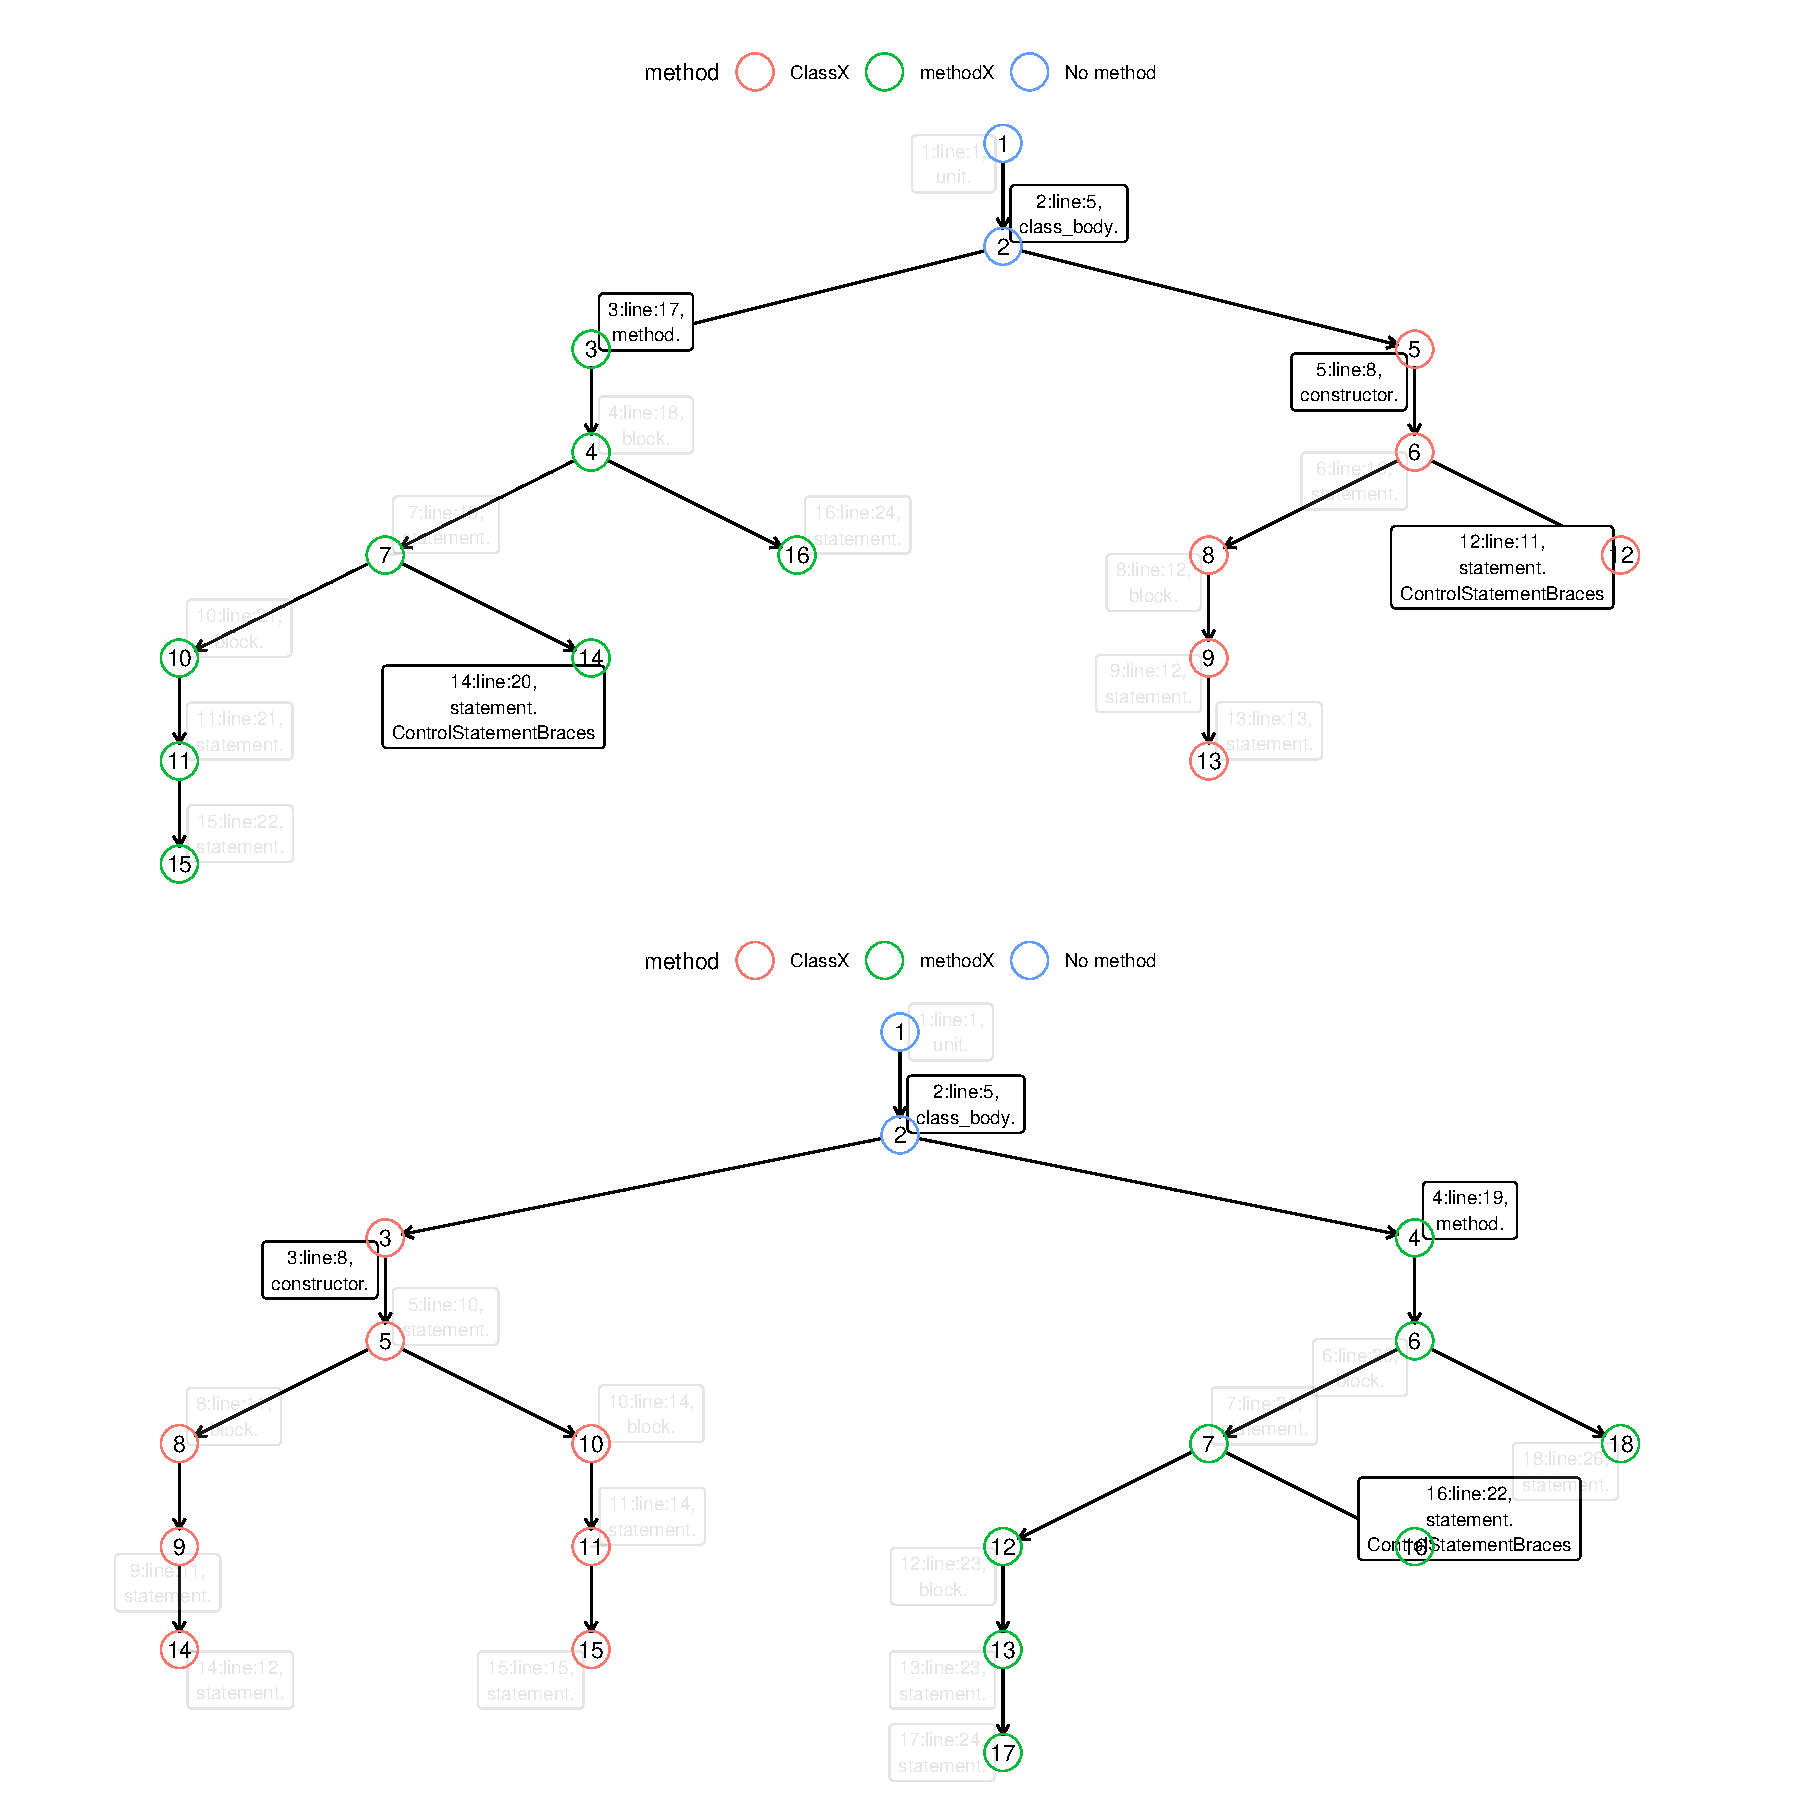
\includegraphics[width=1\linewidth]{report_files/figure-latex/unnamed-chunk-5-1} \caption{Abstract Syntax Trees. New and old versions, with alerts \label{AST_compare_id_alerts}}\label{fig:unnamed-chunk-5}
\end{figure}

\normalsize

\subsection{Map new lines to old lines}\label{map}

For each difference stated in the output of git diff (the sections of
the diff file starting with ``@@''), there is an indication of the
number of lines removed from the old version and the number of lines
added to the new one. The line in which the lines are removed from the
old version and the line at which the lines are added is indicated,
too.\textbackslash{} By using this information we create a relation
between the lines of the old version and the equivalent lines in the new
version. For the new and old versions presented in Section
\ref{source_used}, the relation is shown in Table \ref{table_map}.

\small

\begin{table}[H]

\caption{\label{tab:showing map}Relation between lines of the old version and lines of the new version\label{table_map}}
\centering
\resizebox{\linewidth}{!}{
\begin{tabular}[t]{l|l|l|l|l|l|l|l|l|l|l|l|l|l|l}
\hline
1 & 2 & 3- & -8 & 9 & 10 & \textcolor{white}{7} & 11 & \textcolor{white}{9} & 12 & 13 & 14- & -24 & 25 & 26\\
\hline
1 & 2 & 3- & -8 & 9 & 10 & 11 & 12 & 13 & 14 & 15 & 16- & -26 & 27 & 28\\
\hline
\end{tabular}}
\end{table}

\normalsize

\subsection{Calculate features for each pair of new and old alert}

In the case of the source code we are using as an example, we calculate
features for \(2 \cdot 1 = 2\) combinations of new and old alerts, since
we have 2 old alerts and 1 new alert. The combinations for which the
features must be calculated are shown in Table \ref{combination}

\small

\begin{table}[H]

\caption{\label{tab:unnamed-chunk-6}Combinations of new and old alerts for which the features must be calculated \label{combination}}
\centering
\resizebox{\linewidth}{!}{
\begin{tabular}[t]{r|l|r|l}
\hline
Begin Line Old & Rule Old & Begin Line New & Rule New\\
\hline
11 & ControlStatementBraces & 22 & ControlStatementBraces\\
\hline
20 & ControlStatementBraces & 22 & ControlStatementBraces\\
\hline
\end{tabular}}
\end{table}

\normalsize

We propose the following list of features to calculated for each
combination:

\subsubsection{Same Rule}

A boolean indicator that tells if the alerts are of the same type

\subsubsection{Same Group ID}

A boolean indicator that tells if the alerts are equivalent in terms of
begin line and end line, considering the line map described in Section
\ref{map}.

For each combination, Table \ref{same_group} shows the begin line in the
old version, the corresponding begin line in the new version and the
begin line in the new version
\footnote{we suppress the end lines because for all alerts the begin lines and the old lines are the same}.
We can see that the alert that begins in line 20 of the old version
corresponds to the alert that begins in line 2 of the new version, so,
for this combination the feature ``Same group'' is true. For the other
combination, the feature ``Same Group'' is false.

\small

\begin{table}[H]

\caption{\label{tab:unnamed-chunk-7}Same group feature \label{same_group}}
\centering
\resizebox{\linewidth}{!}{
\begin{tabular}[t]{r|l|r|r|l|l}
\hline
Begin Line Old & Rule Old & Corresponding line in new version & Begin Line New & Rule New & Same group\\
\hline
11 & ControlStatementBraces & 12 & 22 & ControlStatementBraces & FALSE\\
\hline
20 & ControlStatementBraces & 22 & 22 & ControlStatementBraces & TRUE\\
\hline
\end{tabular}}
\end{table}

\normalsize

\subsubsection {Same Method Group ID}

A boolean indicator that tells if the alerts belong to the same method.
We know the alert's method following the path from the alert´s node to
the root. The first node of the kind ``method'' found in this path
defines the alert's method. If this is the same for \(o\) and for \(n\),
then they belong to the same method.

\small

\begin{figure}[H]
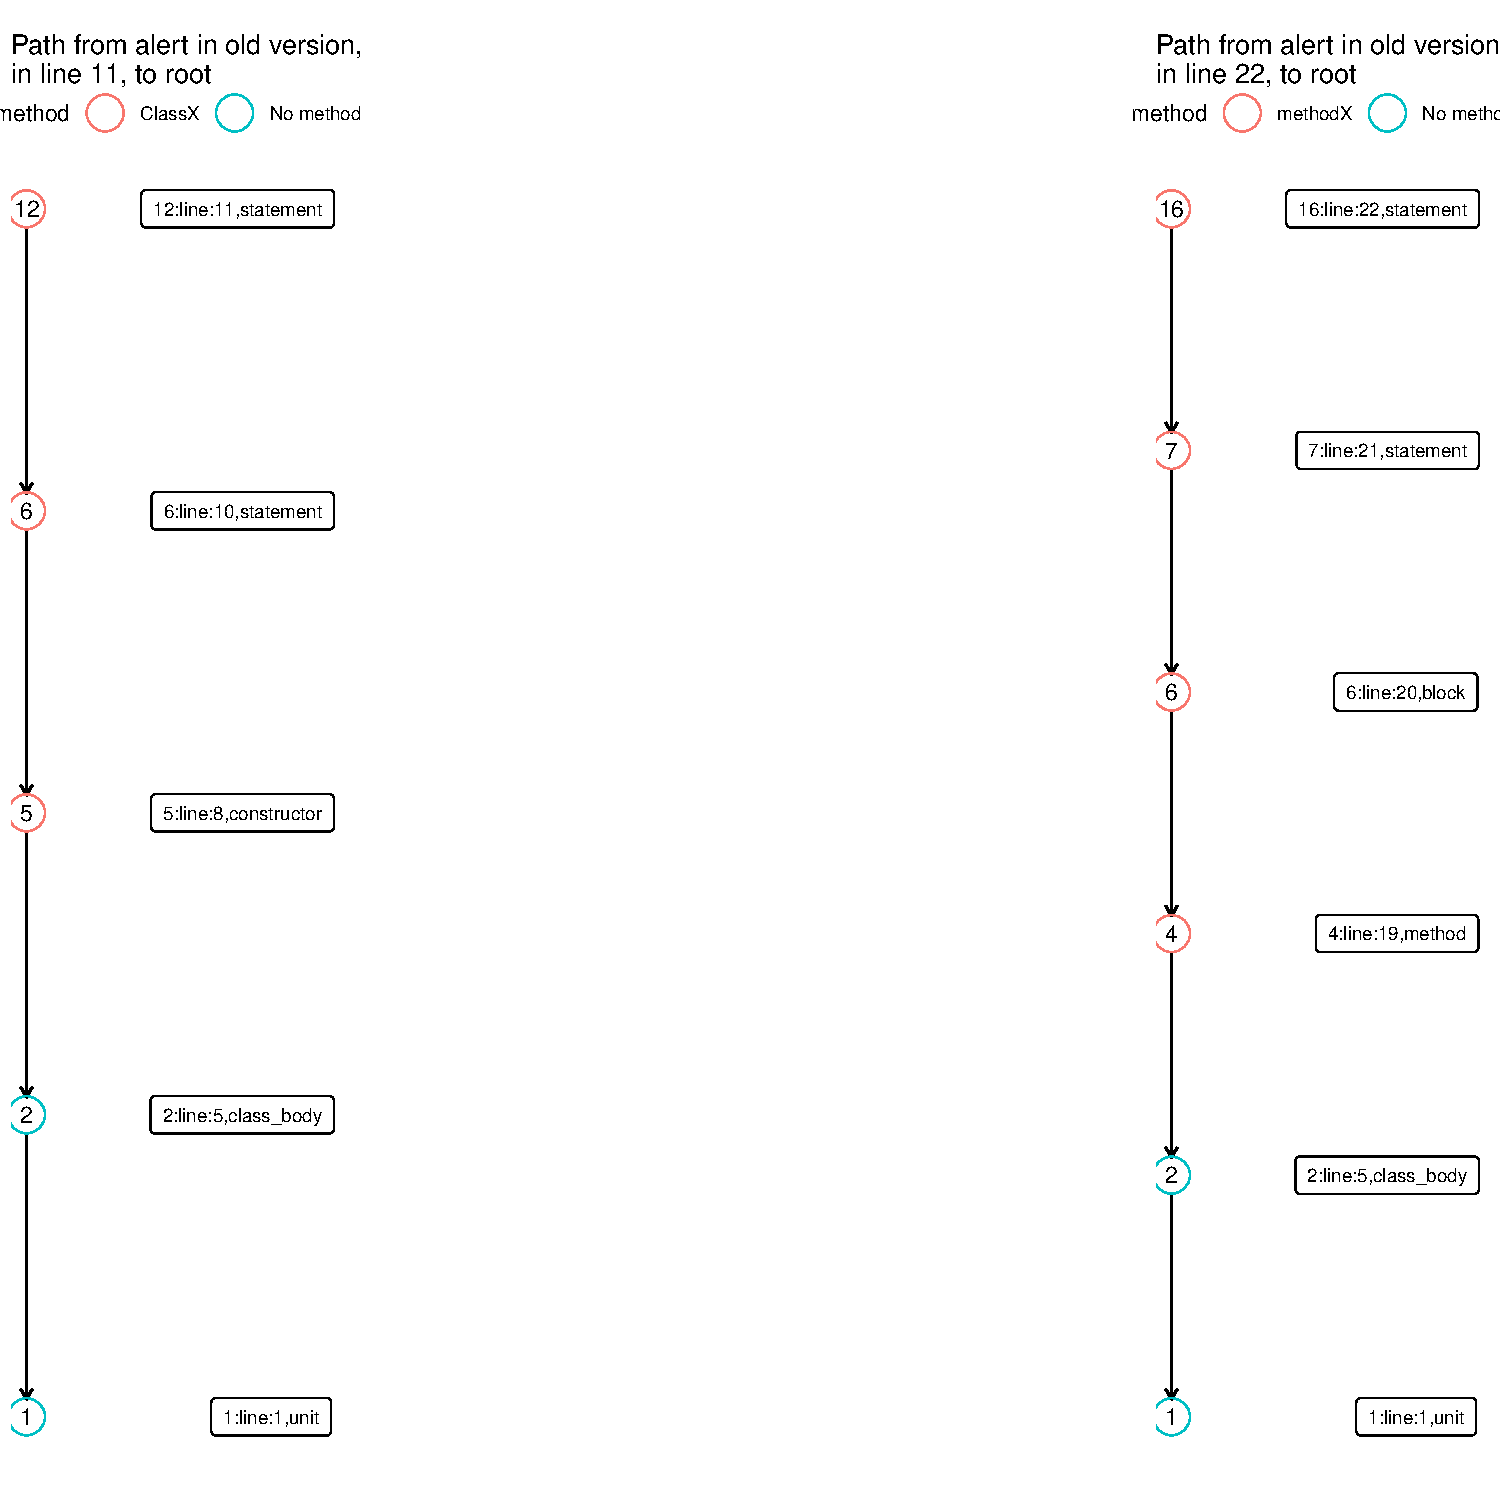
\includegraphics[width=1\linewidth]{report_files/figure-latex/unnamed-chunk-8-1} \caption{Abstract Syntax Tree. Nodes with the same number are equivalent \label{AST_with_alerts}}\label{fig:unnamed-chunk-8}
\end{figure}

\normalsize

Same Method Name: a boolean indicator that tells if the alerts were
found in a method with the same name.

Same Block: a boolean indicator that shows if the \(o\) and \(n\) belong
to the same block. It is defined the same way the ``Same method''
indicator is defined.

Same Code: a boolean indicator that shows the nodes that generate the
alert have the same programming code.

Same Method Code: a boolean indicator that shows that the methods that
contain the nodes that generate the alert have the same programming
code.

Line distance: \(o\) and \(n\) have a begin line \(b(o)\) and \(b(n)\)
and an end line \(e(n)\) and \(e(n)\). Line distance is
\(abs(mean(b(o), e(o)) - mean(b(n), e(n)))\)

Normalized line distance (block size): this is the line distance but
normalized by the size of the last common node.

Normalized line distance (method size): this is the line distance but
normalized by the size of the last common method (if there is no common
method, it´s normalized by the side of the compilation unit).

Normalized line distance (compilation unit size): this is the line
distance but normalized by the size of the compilation unit.

\subsection{Feature engineering} \label{feature_creation}

\begin{itemize}
\item
  Considering the relation between the lines of the two versions constructed as we saw in Section \ref{map}, the nodes in both trees begin and end in related lines;

\item
  The nodes are of the same kind.
\end{itemize}

\small

\begin{figure}[H]
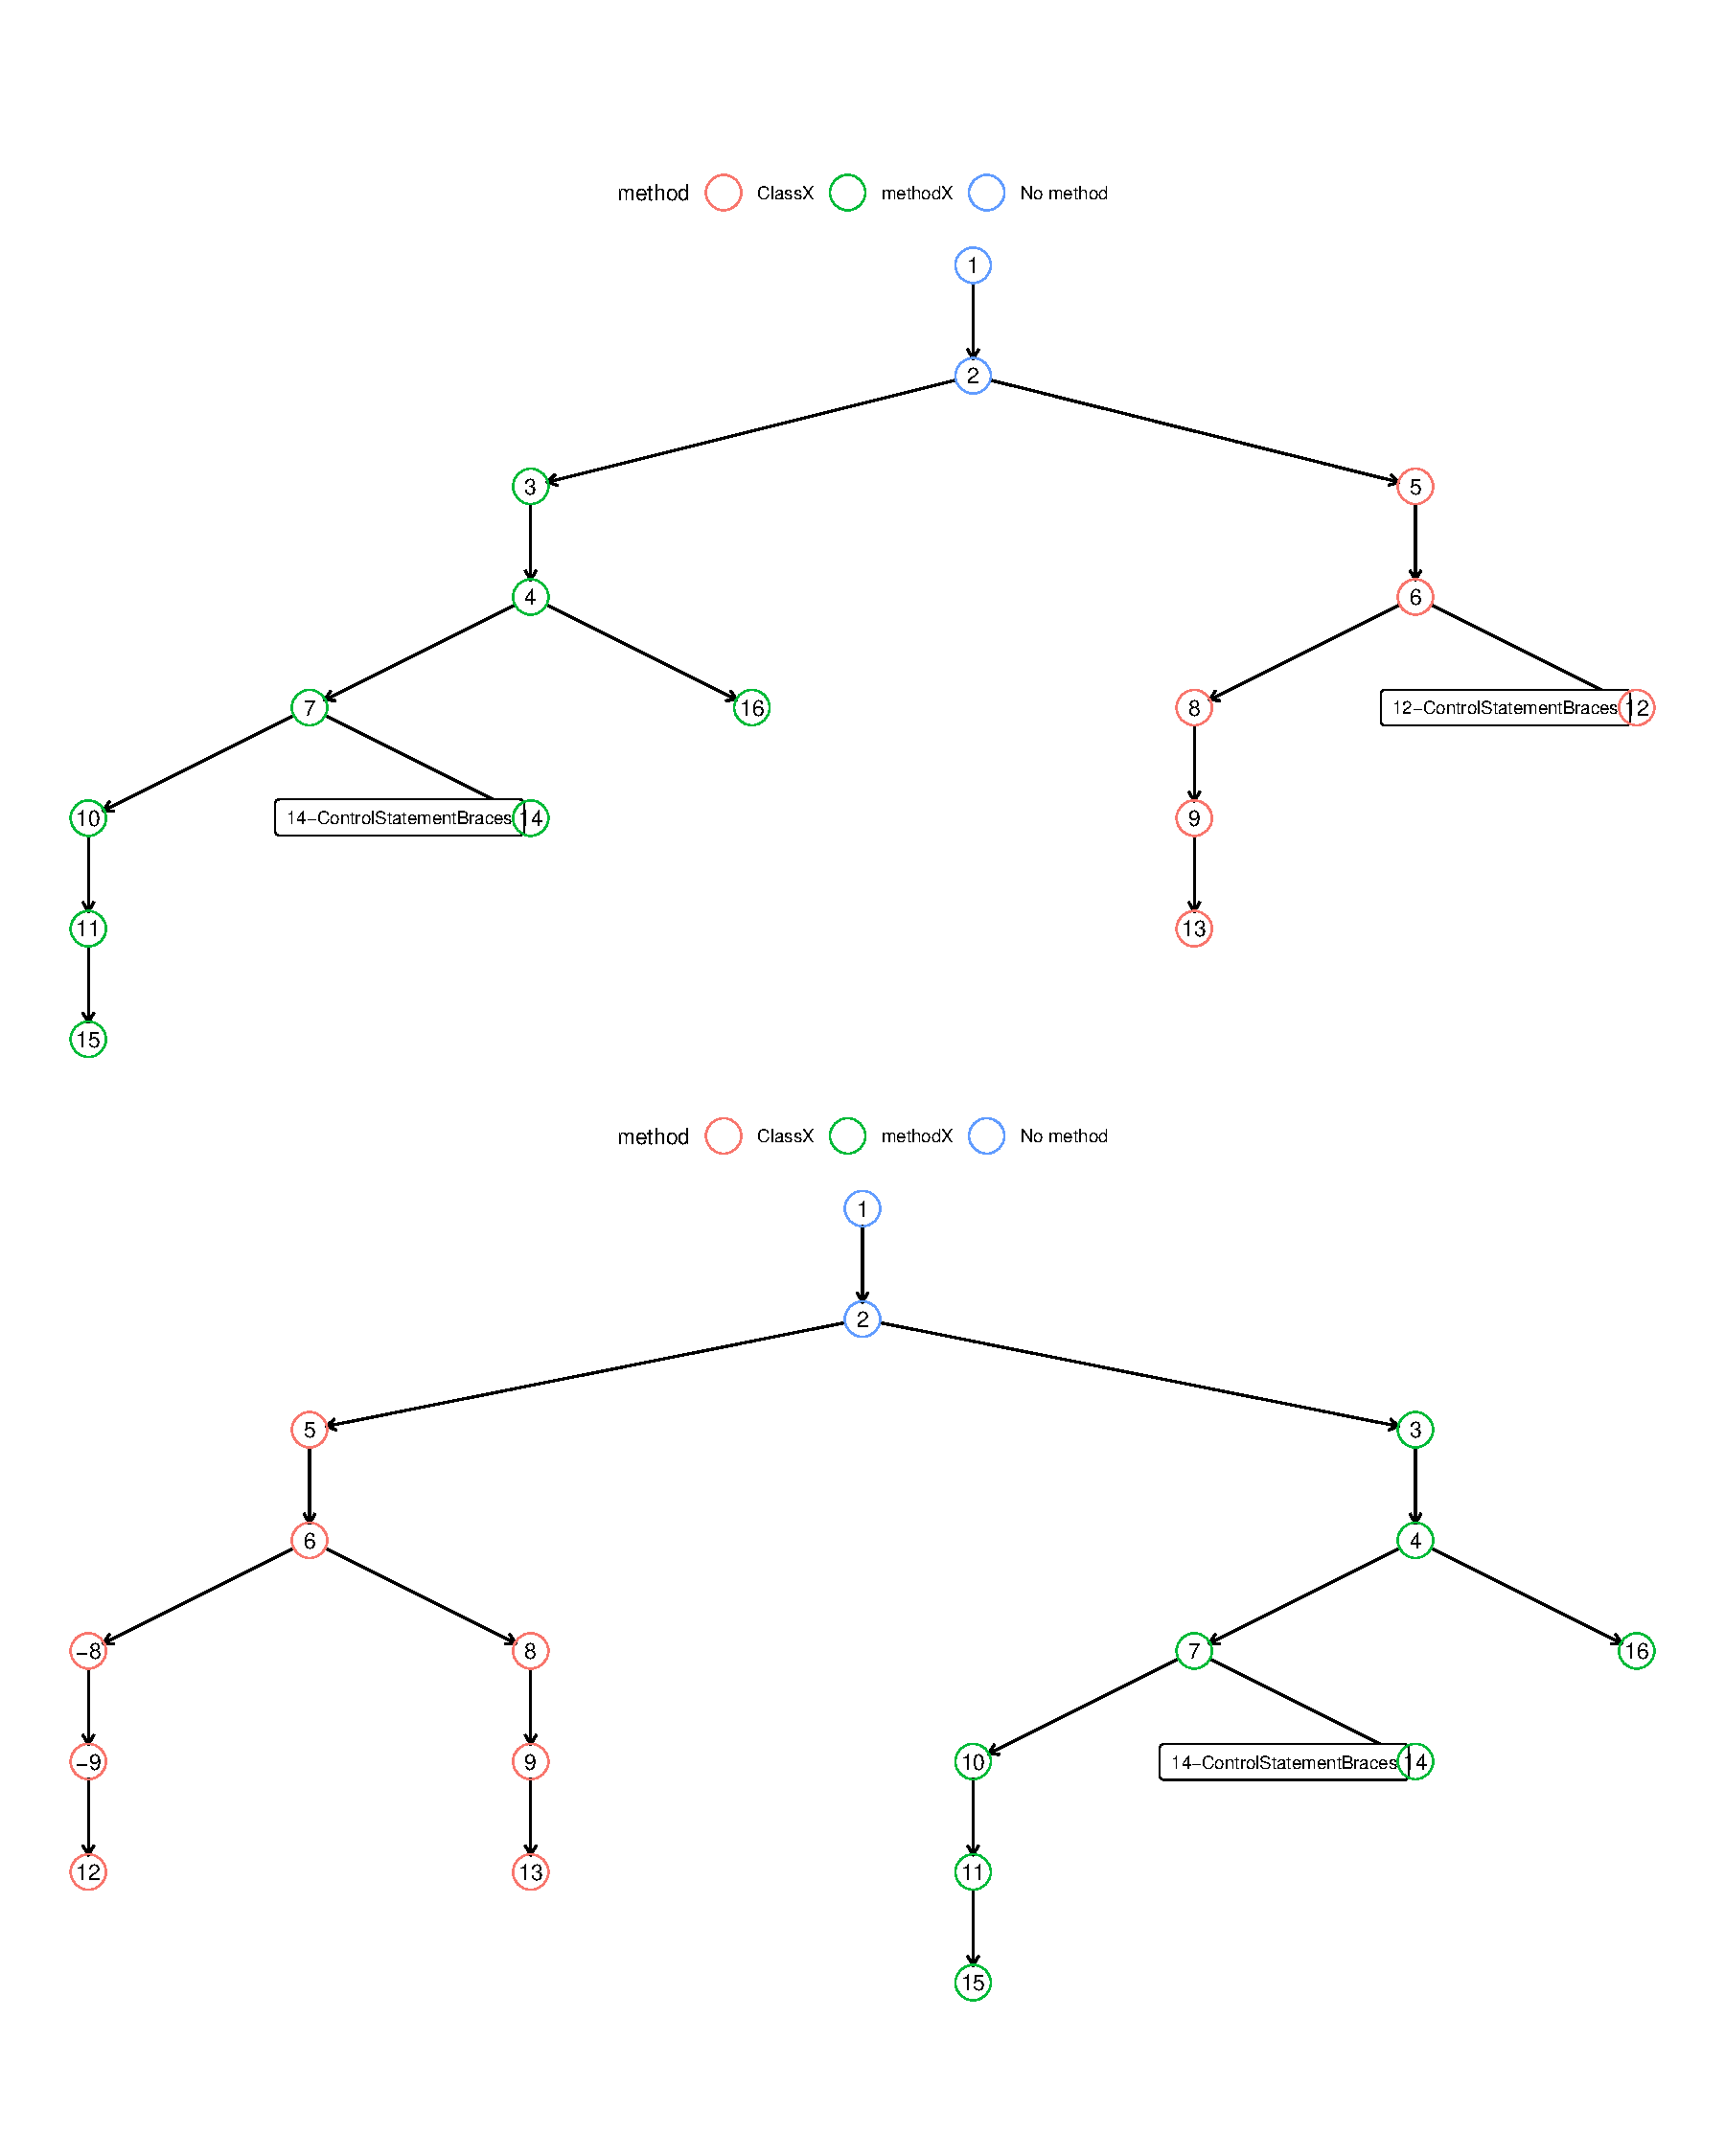
\includegraphics[width=1\linewidth]{report_files/figure-latex/unnamed-chunk-9-1} \caption{Abstract Syntax Tree. Nodes with the same number are equivalent \label{AST_with_alerts}}\label{fig:unnamed-chunk-9}
\end{figure}

\normalsize

The path between the alert and the root of the AST can be seen in
\ref{AST_alert_1}. Comparing the path of different alerts is possible to
determine if the nodes belong to the same method, for instance.

\small

\begin{figure}[H]
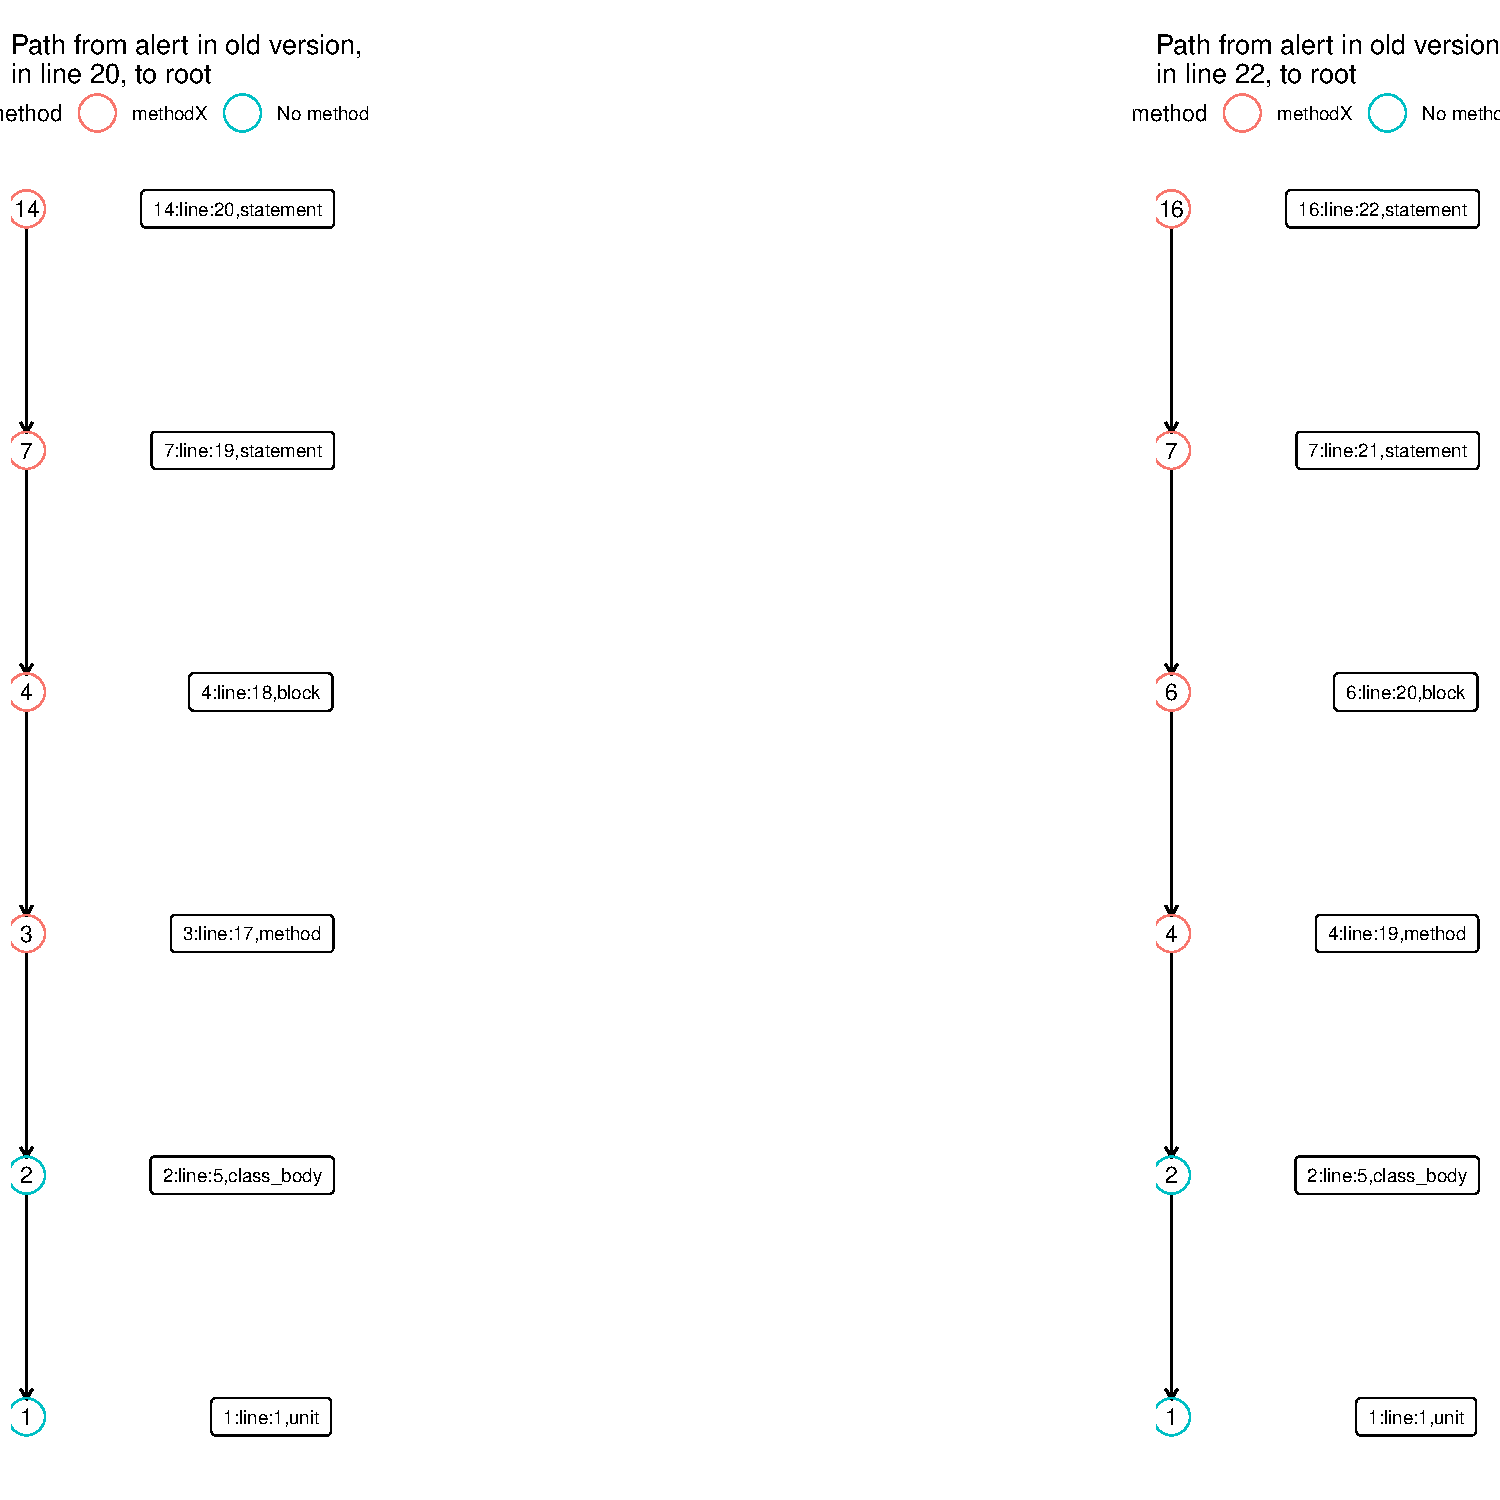
\includegraphics[width=1\linewidth]{report_files/figure-latex/unnamed-chunk-10-1} \caption{Abstract Syntax Tree \label{AST_alert_1}}\label{fig:unnamed-chunk-10}
\end{figure}

\normalsize

The algorithm generates a set of features for each pair of alerts
\((n,o)\) with one element \(n\) coming from the old version and one
element \(o\) coming from the new version. The features do not lead to a
direct conclusion. It´s necessary to create a heuristic or statistical
learning algorithm that will decide the final verdict based on the
features.

We propose the following list of features:

\begin{itemize}
\item
  Same Rule: a boolean indicator that tells if the alerts are of the
  same type
\item
  Same Group ID: a boolean indicator that tells if the alerts are
  equivalent as defined in Figure \ref{AST_groups}
\item
  Same Method Group ID: a boolean indicator that tells if the alerts
  belong to the same method. We know the alert's method following the
  path from the alert´s node to the root. The first node of the kind
  ``method'' found in this path defines the alert's method. If this is
  the same for \(o\) and for \(n\), then they belong to the same method.
\item
  Same Method Name: a boolean indicator that tells if the alerts were
  found in a method with the same name.
\item
  Same Block: a boolean indicator that shows if the \(o\) and \(n\)
  belong to the same block. It is defined the same way the ``Same
  method'' indicator is defined.
\item
  Same Code: a boolean indicator that shows the nodes that generate the
  alert have the same programming code.
\item
  Same Method Code: a boolean indicator that shows that the methods that
  contain the nodes that generate the alert have the same programming
  code.
\item
  Line distance: \(o\) and \(n\) have a begin line \(b(o)\) and \(b(n)\)
  and an end line \(e(n)\) and \(e(n)\). Line distance is
  \(abs(mean(b(o), e(o)) - mean(b(n), e(n)))\)
\item
  Normalized line distance (block size): this is the line distance but
  normalized by the size of the last common node.
\item
  Normalized line distance (method size): this is the line distance but
  normalized by the size of the last common method (if there is no
  common method, it´s normalized by the side of the compilation unit).
\item
  Normalized line distance (compilation unit size): this is the line
  distance but normalized by the size of the compilation unit.
\end{itemize}

Table \ref{table_features} shows the combinations \((n,o)\) in the
example. There are \(2 \cdot 1 = 2\) combinations whereas we have two
alerts in the old version and one alert in the new one.

\small

\begin{table}[!h]

\caption{\label{tab:unnamed-chunk-11}Resulting features\label{table_features} }
\centering
\begin{tabular}[t]{l|l|l}
\hline
Alert combination & Feature & Value\\
\hline
\rowcolor{gray!6}   & Same Rule & TRUE\\

 & Same Group ID & TRUE\\

\rowcolor{gray!6}   & Same Method Group ID & TRUE\\

 & Same Method Name & TRUE\\

\rowcolor{gray!6}   & Same Block & TRUE\\

 & Same Code & TRUE\\

\rowcolor{gray!6}   & Same Method Code & TRUE\\

 & Line Distance & 0.00\\

\rowcolor{gray!6}   & Line Distance Normalized by Block Size & 0.00\\

 & Line Distance Normalized by Method Size & 0.00\\

\multirow[t]{-11}{*}{\raggedright\arraybackslash Line (Old version):20, Line (New version):22} & Line Distance Normalized by Compilation Unit Size & 0.00\\
\hline
\end{tabular}
\end{table}

\normalsize

\small

\normalsize

\newpage

\begin{landscape}

\subsection{Example: Renaming method} \label{example_rename_method}

In this example, the new and old versions have only one alert. The
method in which the alert happens is renamed from MethodX to methodZ.

\scriptsize

\begin{Shaded}
\begin{Highlighting}[]
\CommentTok{/*  1-   */}\KeywordTok{package}\ImportTok{ pack_x;                                          /*  1-   */package pack_x;}                                          
\CommentTok{/*  2-   */}                                                         \CommentTok{/*  2-   */}                                                         
\CommentTok{/*  3-   */}\KeywordTok{import}\ImportTok{ importX.function;                                 /*  3-   */import importX.function;}                                 
\CommentTok{/*  4-   */}                                                         \CommentTok{/*  4-   */}                                                         
\CommentTok{/*  5-   */}\KeywordTok{class}\NormalTok{ ClassX }\KeywordTok{extends}\NormalTok{ ClassY }\KeywordTok{implements}\NormalTok{ InterfX \{         }\CommentTok{/*  5-   */}\KeywordTok{class}\NormalTok{ ClassX }\KeywordTok{extends}\NormalTok{ ClassY }\KeywordTok{implements}\NormalTok{ InterfX \{         }
\CommentTok{/*  6-   */}    \KeywordTok{private} \DataTypeTok{long}\NormalTok{ fieldX;                                 }\CommentTok{/*  6-   */}    \KeywordTok{private} \DataTypeTok{long}\NormalTok{ fieldX;                                 }
\CommentTok{/*  7-   */}                                                         \CommentTok{/*  7-   */}                                                         
\CommentTok{/*  8-   */}    \FunctionTok{ClassX}\NormalTok{(}\DataTypeTok{int}\NormalTok{ paramX, }\DataTypeTok{double}\NormalTok{ paramY) \{                        }\CommentTok{/*  8-   */}    \FunctionTok{ClassX}\NormalTok{(}\DataTypeTok{int}\NormalTok{ paramX, }\DataTypeTok{double}\NormalTok{ paramY) \{                          }
\CommentTok{/*  9-   */}        \DataTypeTok{int}\NormalTok{ varX = }\FunctionTok{function}\NormalTok{(paramX, paramY);                  }\CommentTok{/*  9-   */}        \DataTypeTok{int}\NormalTok{ varX = }\FunctionTok{function}\NormalTok{(paramX, paramY);                     }
\CommentTok{/*   -   *//*XXXXXXXXXXXXXXXXXXXXXXXXXXXXXXXXXXXXXX*/}               \CommentTok{/* 10-   */}        \KeywordTok{if}\NormalTok{ (varX == }\DecValTok{0}\NormalTok{)                                   }
\CommentTok{/* 10-   */}        \KeywordTok{if}\NormalTok{ (varX == }\DecValTok{0}\NormalTok{)\{                                  }\CommentTok{/*   -   *//*XXXXXXXXXXXXXXXXXXXXXXXXXXXXXXXXXXXXXX*/}               
\CommentTok{/*   -   *//*XXXXXXXXXXXXXXXXXXXXXXXXXXXXXXXXXXXXXX*/}               \CommentTok{/* 11-   */}\NormalTok{        \{                                                }
\CommentTok{/* 11-   */}            \KeywordTok{this}\NormalTok{.}\FunctionTok{fieldX}\NormalTok{ = }\DecValTok{1}\NormalTok{;                             }\CommentTok{/* 12-   */}            \KeywordTok{this}\NormalTok{.}\FunctionTok{fieldX}\NormalTok{ = }\DecValTok{1}\NormalTok{;                             }
\CommentTok{/* 12-   */}\NormalTok{        \}                                                }\CommentTok{/*   -   *//*XXXXXXXXXXXXXXXXXXXXXXXXXXXXXXXXXXXXXX*/}               
\CommentTok{/*   -   *//*XXXXXXXXXXXXXXXXXXXXXXXXXXXXXXXXXXXXXX*/}               \CommentTok{/* 13-   */}\NormalTok{        \}                                                            }
\CommentTok{/* 13-   */}        \KeywordTok{else}\NormalTok{\{                                            }\CommentTok{/* 14-   */}        \KeywordTok{else}\NormalTok{\{                                            }
\CommentTok{/* 14-   */}            \KeywordTok{this}\NormalTok{.}\FunctionTok{fieldX}\NormalTok{ = }\DecValTok{0}\NormalTok{;                             }\CommentTok{/* 15-   */}            \KeywordTok{this}\NormalTok{.}\FunctionTok{fieldX}\NormalTok{ = }\DecValTok{0}\NormalTok{;                             }
\CommentTok{/* 15-   */}\NormalTok{        \}                                                }\CommentTok{/* 16-   */}\NormalTok{        \}                                                }
\CommentTok{/* 16-   */}\NormalTok{    \}                                                    }\CommentTok{/* 17-   */}\NormalTok{    \}                                                    }
\CommentTok{/* 17-   */}    \AttributeTok{@Override}                                            \CommentTok{/* 18-   */}    \AttributeTok{@Override}                                            
\CommentTok{/* 18-   */}    \KeywordTok{public} \DataTypeTok{int} \FunctionTok{methodX}\NormalTok{(}\DataTypeTok{int}\NormalTok{ paramW, }\BuiltInTok{Boolean}\NormalTok{ paramZ)       }\CommentTok{/*   -   *//*XXXXXXXXXXXXXXXXXXXXXXXXXXXXXXXXXXXXXX*/}               
\CommentTok{/*   -   *//*XXXXXXXXXXXXXXXXXXXXXXXXXXXXXXXXXXXXXX*/}               \CommentTok{/* 19-   */}    \KeywordTok{public} \DataTypeTok{int} \FunctionTok{methodZ}\NormalTok{(}\DataTypeTok{int}\NormalTok{ paramW, }\BuiltInTok{Boolean}\NormalTok{ paramZ)       }
\CommentTok{/* 19-   */}\NormalTok{    \{                                                    }\CommentTok{/* 20-   */}\NormalTok{    \{                                                    }
\CommentTok{/* 20-   */}        \KeywordTok{if}\NormalTok{ (paramZ)                                      }\CommentTok{/* 21-   */}        \KeywordTok{if}\NormalTok{ (paramZ)                                      }
\CommentTok{/* 21-CSB*/}\NormalTok{            fieldX = paramW;                             }\CommentTok{/* 22-CSB*/}\NormalTok{            fieldX = paramW;                             }
\CommentTok{/* 22-   */}        \KeywordTok{else}\NormalTok{\{                                            }\CommentTok{/* 23-   */}        \KeywordTok{else}\NormalTok{\{                                            }
\CommentTok{/* 23-   */}\NormalTok{            fieldX = }\DecValTok{0}\NormalTok{;                                  }\CommentTok{/* 24-   */}\NormalTok{            fieldX = }\DecValTok{0}\NormalTok{;                                  }
\CommentTok{/* 24-   */}\NormalTok{        \}                                                }\CommentTok{/* 25-   */}\NormalTok{        \}                                                }
\CommentTok{/* 25-   */}        \KeywordTok{return}\NormalTok{ paramW + }\KeywordTok{this}\NormalTok{.}\FunctionTok{fieldX}\NormalTok{;                     }\CommentTok{/* 26-   */}        \KeywordTok{return}\NormalTok{ paramW + }\KeywordTok{this}\NormalTok{.}\FunctionTok{fieldX}\NormalTok{;                     }
\CommentTok{/* 26-   */}\NormalTok{     \}                                                   }\CommentTok{/* 27-   */}\NormalTok{     \}                                                   }
\CommentTok{/* 27-   */}\NormalTok{\}                                                        }\CommentTok{/* 28-   */}\NormalTok{\}                                                        }


\NormalTok{CSB: ControlStatementBraces}
\end{Highlighting}
\end{Shaded}

\normalsize

\begin{figure}
\centering

\includegraphics{figures/fake.png}
\caption{Comparison between old and new version
\label{comparison_rename}}
\end{figure}

\end{landscape}

\newpage

In the Table \ref{features_rename} we can see that the features ``Same
Method Name'' and ``Same Method Group ID'' are now FALSE.

\small

\begin{table}[!h]

\caption{\label{tab:unnamed-chunk-13}Resulting features: rename method example \label{features_rename} }
\centering
\begin{tabular}[t]{l|l|l}
\hline
Alert combination & Feature & Value\\
\hline
\rowcolor{gray!6}   & Same Rule & TRUE\\

 & Same Group ID & TRUE\\

\rowcolor{gray!6}   & Same Method Group ID & FALSE\\

 & Same Method Name & FALSE\\

\rowcolor{gray!6}   & Same Block & TRUE\\

 & Same Code & TRUE\\

\rowcolor{gray!6}   & Same Method Code & FALSE\\

 & Line Distance & 0.00\\

\rowcolor{gray!6}   & Line Distance Normalized by Block Size & 0.00\\

 & Line Distance Normalized by Method Size & 0.00\\

\multirow[t]{-11}{*}{\raggedright\arraybackslash Line (Old version):21, Line (New version):22} & Line Distance Normalized by Compilation Unit Size & 0.00\\
\hline
\end{tabular}
\end{table}

\normalsize

\newpage

\begin{landscape}

\subsection{Example: including a statement before} \label{example_including_statement}

\small

\normalsize

In this example, a new statement is included before the alert.

\small

\normalsize

\scriptsize

\begin{Shaded}
\begin{Highlighting}[]
\CommentTok{/*  1-   */}\KeywordTok{package}\ImportTok{ pack_x;                                          /*  1-   */package pack_x;}                                          
\CommentTok{/*  2-   */}                                                         \CommentTok{/*  2-   */}                                                         
\CommentTok{/*  3-   */}\KeywordTok{import}\ImportTok{ importX.function;                                 /*  3-   */import importX.function;}                                 
\CommentTok{/*  4-   */}                                                         \CommentTok{/*  4-   */}                                                         
\CommentTok{/*  5-   */}\KeywordTok{class}\NormalTok{ ClassX }\KeywordTok{extends}\NormalTok{ ClassY }\KeywordTok{implements}\NormalTok{ InterfX \{         }\CommentTok{/*  5-   */}\KeywordTok{class}\NormalTok{ ClassX }\KeywordTok{extends}\NormalTok{ ClassY }\KeywordTok{implements}\NormalTok{ InterfX \{         }
\CommentTok{/*  6-   */}    \KeywordTok{private} \DataTypeTok{long}\NormalTok{ fieldX;                                 }\CommentTok{/*  6-   */}    \KeywordTok{private} \DataTypeTok{long}\NormalTok{ fieldX;                                 }
\CommentTok{/*  7-   */}                                                         \CommentTok{/*  7-   */}                                                         
\CommentTok{/*  8-   */}    \FunctionTok{ClassX}\NormalTok{(}\DataTypeTok{int}\NormalTok{ paramX, }\DataTypeTok{double}\NormalTok{ paramY) \{                        }\CommentTok{/*  8-   */}    \FunctionTok{ClassX}\NormalTok{(}\DataTypeTok{int}\NormalTok{ paramX, }\DataTypeTok{double}\NormalTok{ paramY) \{                          }
\CommentTok{/*  9-   */}        \DataTypeTok{int}\NormalTok{ varX = }\FunctionTok{function}\NormalTok{(paramX, paramY);                  }\CommentTok{/*  9-   */}        \DataTypeTok{int}\NormalTok{ varX = }\FunctionTok{function}\NormalTok{(paramX, paramY);                     }
\CommentTok{/*   -   *//*XXXXXXXXXXXXXXXXXXXXXXXXXXXXXXXXXXXXXX*/}               \CommentTok{/* 10-   */}        \KeywordTok{if}\NormalTok{ (varX == }\DecValTok{0}\NormalTok{)                                   }
\CommentTok{/* 10-   */}        \KeywordTok{if}\NormalTok{ (varX == }\DecValTok{0}\NormalTok{)\{                                  }\CommentTok{/*   -   *//*XXXXXXXXXXXXXXXXXXXXXXXXXXXXXXXXXXXXXX*/}               
\CommentTok{/*   -   *//*XXXXXXXXXXXXXXXXXXXXXXXXXXXXXXXXXXXXXX*/}               \CommentTok{/* 11-   */}\NormalTok{        \{                                                }
\CommentTok{/* 11-   */}            \KeywordTok{this}\NormalTok{.}\FunctionTok{fieldX}\NormalTok{ = }\DecValTok{1}\NormalTok{;                             }\CommentTok{/* 12-   */}            \KeywordTok{this}\NormalTok{.}\FunctionTok{fieldX}\NormalTok{ = }\DecValTok{1}\NormalTok{;                             }
\CommentTok{/* 12-   */}\NormalTok{        \}                                                }\CommentTok{/*   -   *//*XXXXXXXXXXXXXXXXXXXXXXXXXXXXXXXXXXXXXX*/}               
\CommentTok{/*   -   *//*XXXXXXXXXXXXXXXXXXXXXXXXXXXXXXXXXXXXXX*/}               \CommentTok{/* 13-   */}\NormalTok{        \}                                                            }
\CommentTok{/* 13-   */}        \KeywordTok{else}\NormalTok{\{                                            }\CommentTok{/* 14-   */}        \KeywordTok{else}\NormalTok{\{                                            }
\CommentTok{/* 14-   */}            \KeywordTok{this}\NormalTok{.}\FunctionTok{fieldX}\NormalTok{ = }\DecValTok{0}\NormalTok{;                             }\CommentTok{/* 15-   */}            \KeywordTok{this}\NormalTok{.}\FunctionTok{fieldX}\NormalTok{ = }\DecValTok{0}\NormalTok{;                             }
\CommentTok{/* 15-   */}\NormalTok{        \}                                                }\CommentTok{/* 16-   */}\NormalTok{        \}                                                }
\CommentTok{/* 16-   */}\NormalTok{    \}                                                    }\CommentTok{/* 17-   */}\NormalTok{    \}                                                    }
\CommentTok{/* 17-   */}    \AttributeTok{@Override}                                            \CommentTok{/* 18-   */}    \AttributeTok{@Override}                                            
\CommentTok{/* 18-   */}    \KeywordTok{public} \DataTypeTok{int} \FunctionTok{methodX}\NormalTok{(}\DataTypeTok{int}\NormalTok{ paramW, }\BuiltInTok{Boolean}\NormalTok{ paramZ)       }\CommentTok{/* 19-   */}    \KeywordTok{public} \DataTypeTok{int} \FunctionTok{methodX}\NormalTok{(}\DataTypeTok{int}\NormalTok{ paramW, }\BuiltInTok{Boolean}\NormalTok{ paramZ)       }
\CommentTok{/* 19-   */}\NormalTok{    \{                                                    }\CommentTok{/* 20-   */}\NormalTok{    \{                                                    }
\CommentTok{/*   -   *//*XXXXXXXXXXXXXXXXXXXXXXXXXXXXXXXXXXXXXX*/}               \CommentTok{/* 21-   */}\NormalTok{        paramT = }\DecValTok{0}\NormalTok{;                                      }
\CommentTok{/* 20-   */}        \KeywordTok{if}\NormalTok{ (paramZ)                                      }\CommentTok{/* 22-   */}        \KeywordTok{if}\NormalTok{ (paramZ)                                      }
\CommentTok{/* 21-CSB*/}\NormalTok{            fieldX = paramW;                             }\CommentTok{/* 23-CSB*/}\NormalTok{            fieldX = paramW;                             }
\CommentTok{/* 22-   */}        \KeywordTok{else}\NormalTok{\{                                            }\CommentTok{/* 24-   */}        \KeywordTok{else}\NormalTok{\{                                            }
\CommentTok{/* 23-   */}\NormalTok{            fieldX = }\DecValTok{0}\NormalTok{;                                  }\CommentTok{/* 25-   */}\NormalTok{            fieldX = }\DecValTok{0}\NormalTok{;                                  }
\CommentTok{/* 24-   */}\NormalTok{        \}                                                }\CommentTok{/* 26-   */}\NormalTok{        \}                                                }
\CommentTok{/* 25-   */}        \KeywordTok{return}\NormalTok{ paramW + }\KeywordTok{this}\NormalTok{.}\FunctionTok{fieldX}\NormalTok{;                     }\CommentTok{/* 27-   */}        \KeywordTok{return}\NormalTok{ paramW + }\KeywordTok{this}\NormalTok{.}\FunctionTok{fieldX}\NormalTok{;                     }
\CommentTok{/* 26-   */}\NormalTok{     \}                                                   }\CommentTok{/* 28-   */}\NormalTok{     \}                                                   }
\CommentTok{/* 27-   */}\NormalTok{\}                                                        }\CommentTok{/* 29-   */}\NormalTok{\}                                                        }


\NormalTok{CSB: ControlStatementBraces}
\end{Highlighting}
\end{Shaded}

\normalsize

\begin{figure}
\centering

\includegraphics{figures/fake.png}
\caption{Comparison between old and new version
\label{comparison_include_statement_before}}
\end{figure}

\end{landscape}

\newpage

In the Table \ref{include_statement_before} we can see that the features
are not affected by this new statement.

\small

\begin{table}[!h]

\caption{\label{tab:unnamed-chunk-16}Resulting features: statement included before \label{include_statement_before} }
\centering
\begin{tabular}[t]{l|l|l}
\hline
Alert combination & Feature & Value\\
\hline
\rowcolor{gray!6}   & Same Rule & TRUE\\

 & Same Group ID & TRUE\\

\rowcolor{gray!6}   & Same Method Group ID & TRUE\\

 & Same Method Name & TRUE\\

\rowcolor{gray!6}   & Same Block & TRUE\\

 & Same Code & TRUE\\

\rowcolor{gray!6}   & Same Method Code & FALSE\\

 & Line Distance & 0.00\\

\rowcolor{gray!6}   & Line Distance Normalized by Block Size & 0.00\\

 & Line Distance Normalized by Method Size & 0.00\\

\multirow[t]{-11}{*}{\raggedright\arraybackslash Line (Old version):21, Line (New version):23} & Line Distance Normalized by Compilation Unit Size & 0.00\\
\hline
\end{tabular}
\end{table}

\normalsize

\newpage

\begin{landscape}

\subsection{Example: nesting the alert in an if statement} \label{example_nested_in_other_if}

\small

\normalsize

\scriptsize

\begin{Shaded}
\begin{Highlighting}[]
\CommentTok{/*  1-   */}\KeywordTok{package}\ImportTok{ pack_x;                                          /*  1-   */package pack_x;}                                          
\CommentTok{/*  2-   */}                                                         \CommentTok{/*  2-   */}                                                         
\CommentTok{/*  3-   */}\KeywordTok{import}\ImportTok{ importX.function;                                 /*  3-   */import importX.function;}                                 
\CommentTok{/*  4-   */}                                                         \CommentTok{/*  4-   */}                                                         
\CommentTok{/*  5-   */}\KeywordTok{class}\NormalTok{ ClassX }\KeywordTok{extends}\NormalTok{ ClassY }\KeywordTok{implements}\NormalTok{ InterfX \{         }\CommentTok{/*  5-   */}\KeywordTok{class}\NormalTok{ ClassX }\KeywordTok{extends}\NormalTok{ ClassY }\KeywordTok{implements}\NormalTok{ InterfX \{         }
\CommentTok{/*  6-   */}    \KeywordTok{private} \DataTypeTok{long}\NormalTok{ fieldX;                                 }\CommentTok{/*  6-   */}    \KeywordTok{private} \DataTypeTok{long}\NormalTok{ fieldX;                                 }
\CommentTok{/*  7-   */}                                                         \CommentTok{/*  7-   */}                                                         
\CommentTok{/*  8-   */}    \FunctionTok{ClassX}\NormalTok{(}\DataTypeTok{int}\NormalTok{ paramX, }\DataTypeTok{double}\NormalTok{ paramY) \{                        }\CommentTok{/*  8-   */}    \FunctionTok{ClassX}\NormalTok{(}\DataTypeTok{int}\NormalTok{ paramX, }\DataTypeTok{double}\NormalTok{ paramY) \{                          }
\CommentTok{/*  9-   */}        \DataTypeTok{int}\NormalTok{ varX = }\FunctionTok{function}\NormalTok{(paramX, paramY);                  }\CommentTok{/*  9-   */}        \DataTypeTok{int}\NormalTok{ varX = }\FunctionTok{function}\NormalTok{(paramX, paramY);                     }
\CommentTok{/*   -   *//*XXXXXXXXXXXXXXXXXXXXXXXXXXXXXXXXXXXXXX*/}               \CommentTok{/* 10-   */}        \KeywordTok{if}\NormalTok{ (varX == }\DecValTok{0}\NormalTok{)                                   }
\CommentTok{/* 10-   */}        \KeywordTok{if}\NormalTok{ (varX == }\DecValTok{0}\NormalTok{)\{                                  }\CommentTok{/*   -   *//*XXXXXXXXXXXXXXXXXXXXXXXXXXXXXXXXXXXXXX*/}               
\CommentTok{/*   -   *//*XXXXXXXXXXXXXXXXXXXXXXXXXXXXXXXXXXXXXX*/}               \CommentTok{/* 11-   */}\NormalTok{        \{                                                }
\CommentTok{/* 11-   */}            \KeywordTok{this}\NormalTok{.}\FunctionTok{fieldX}\NormalTok{ = }\DecValTok{1}\NormalTok{;                             }\CommentTok{/* 12-   */}            \KeywordTok{this}\NormalTok{.}\FunctionTok{fieldX}\NormalTok{ = }\DecValTok{1}\NormalTok{;                             }
\CommentTok{/* 12-   */}\NormalTok{        \}                                                }\CommentTok{/*   -   *//*XXXXXXXXXXXXXXXXXXXXXXXXXXXXXXXXXXXXXX*/}               
\CommentTok{/*   -   *//*XXXXXXXXXXXXXXXXXXXXXXXXXXXXXXXXXXXXXX*/}               \CommentTok{/* 13-   */}\NormalTok{        \}                                                            }
\CommentTok{/* 13-   */}        \KeywordTok{else}\NormalTok{\{                                            }\CommentTok{/* 14-   */}        \KeywordTok{else}\NormalTok{\{                                            }
\CommentTok{/* 14-   */}            \KeywordTok{this}\NormalTok{.}\FunctionTok{fieldX}\NormalTok{ = }\DecValTok{0}\NormalTok{;                             }\CommentTok{/* 15-   */}            \KeywordTok{this}\NormalTok{.}\FunctionTok{fieldX}\NormalTok{ = }\DecValTok{0}\NormalTok{;                             }
\CommentTok{/* 15-   */}\NormalTok{        \}                                                }\CommentTok{/* 16-   */}\NormalTok{        \}                                                }
\CommentTok{/* 16-   */}\NormalTok{    \}                                                    }\CommentTok{/* 17-   */}\NormalTok{    \}                                                    }
\CommentTok{/* 17-   */}    \AttributeTok{@Override}                                            \CommentTok{/* 18-   */}    \AttributeTok{@Override}                                            
\CommentTok{/* 18-   */}    \KeywordTok{public} \DataTypeTok{int} \FunctionTok{methodX}\NormalTok{(}\DataTypeTok{int}\NormalTok{ paramW, }\BuiltInTok{Boolean}\NormalTok{ paramZ)       }\CommentTok{/* 19-   */}    \KeywordTok{public} \DataTypeTok{int} \FunctionTok{methodX}\NormalTok{(}\DataTypeTok{int}\NormalTok{ paramW, }\BuiltInTok{Boolean}\NormalTok{ paramZ)       }
\CommentTok{/* 19-   */}\NormalTok{    \{                                                    }\CommentTok{/* 20-   */}\NormalTok{    \{                                                    }
\CommentTok{/* 20-   */}        \KeywordTok{if}\NormalTok{ (paramZ)                                      }\CommentTok{/*   -   *//*XXXXXXXXXXXXXXXXXXXXXXXXXXXXXXXXXXXXXX*/}               
\CommentTok{/*   -   *//*XXXXXXXXXXXXXXXXXXXXXXXXXXXXXXXXXXXXXX*/}               \CommentTok{/* 21-   */}        \KeywordTok{if}\NormalTok{(paramZ == }\DecValTok{0}\NormalTok{)\{                                 }
\CommentTok{/* 21-CSB*/}\NormalTok{            fieldX = paramW;                             }\CommentTok{/*   -   *//*XXXXXXXXXXXXXXXXXXXXXXXXXXXXXXXXXXXXXX*/}               
\CommentTok{/*   -   *//*XXXXXXXXXXXXXXXXXXXXXXXXXXXXXXXXXXXXXX*/}               \CommentTok{/* 22-   */}            \KeywordTok{if}\NormalTok{ (paramZ)                                  }
\CommentTok{/*   -   *//*XXXXXXXXXXXXXXXXXXXXXXXXXXXXXXXXXXXXXX*/}               \CommentTok{/* 23-CSB*/}\NormalTok{                fieldX = paramW;                         }
\CommentTok{/* 23-   */}\NormalTok{            fieldX = }\DecValTok{0}\NormalTok{;                                  }\CommentTok{/*   -   *//*XXXXXXXXXXXXXXXXXXXXXXXXXXXXXXXXXXXXXX*/}               
\CommentTok{/*   -   *//*XXXXXXXXXXXXXXXXXXXXXXXXXXXXXXXXXXXXXX*/}               \CommentTok{/* 24-   */}            \KeywordTok{else}\NormalTok{\{                                        }
\CommentTok{/*   -   *//*XXXXXXXXXXXXXXXXXXXXXXXXXXXXXXXXXXXXXX*/}               \CommentTok{/* 25-   */}\NormalTok{                fieldX = }\DecValTok{0}\NormalTok{;                              }
\CommentTok{/*   -   *//*XXXXXXXXXXXXXXXXXXXXXXXXXXXXXXXXXXXXXX*/}               \CommentTok{/* 26-   */}\NormalTok{            \}                                            }
\CommentTok{/*   -   *//*XXXXXXXXXXXXXXXXXXXXXXXXXXXXXXXXXXXXXX*/}               \CommentTok{/* 27-   */}\NormalTok{        \}                                                }
\CommentTok{/* 22-   */}        \KeywordTok{else}\NormalTok{\{                                            }\CommentTok{/* 28-   */}        \KeywordTok{else}\NormalTok{\{                                            }
\CommentTok{/*   -   *//*XXXXXXXXXXXXXXXXXXXXXXXXXXXXXXXXXXXXXX*/}               \CommentTok{/* 29-   */}\NormalTok{            fieldX = }\DecValTok{1}\NormalTok{;                                  }
\CommentTok{/* 24-   */}\NormalTok{        \}                                                }\CommentTok{/* 30-   */}\NormalTok{        \}                                                }
\CommentTok{/* 25-   */}        \KeywordTok{return}\NormalTok{ paramW + }\KeywordTok{this}\NormalTok{.}\FunctionTok{fieldX}\NormalTok{;                     }\CommentTok{/* 31-   */}        \KeywordTok{return}\NormalTok{ paramW + }\KeywordTok{this}\NormalTok{.}\FunctionTok{fieldX}\NormalTok{;                     }
\CommentTok{/* 26-   */}\NormalTok{     \}                                                   }\CommentTok{/* 32-   */}\NormalTok{     \}                                                   }
\CommentTok{/* 27-   */}\NormalTok{\}                                                        }\CommentTok{/* 33-   */}\NormalTok{\}                                                        }


\NormalTok{CSB: ControlStatementBraces}
\end{Highlighting}
\end{Shaded}

\normalsize

\begin{figure}
\centering

\includegraphics{figures/fake.png}
\caption{Comparison between old and new version
\label{comparison_nested_in_other_if}}
\end{figure}

\end{landscape}

\newpage

In the Table \ref{nested_in_other_if} we can see that the algorithm does
not recognize the two nodes as equivalent, but other features can lead
us to the conclusion that the alert is still open.

\small

\begin{table}[!h]

\caption{\label{tab:unnamed-chunk-18}Resulting features: statement included before \label{nested_in_other_if} }
\centering
\begin{tabular}[t]{l|l|l}
\hline
Alert combination & Feature & Value\\
\hline
\rowcolor{gray!6}   & Same Rule & TRUE\\

 & Same Group ID & FALSE\\

\rowcolor{gray!6}   & Same Method Group ID & TRUE\\

 & Same Method Name & TRUE\\

\rowcolor{gray!6}   & Same Block & FALSE\\

 & Same Code & TRUE\\

\rowcolor{gray!6}   & Same Method Code & FALSE\\

 & Line Distance & 2.00\\

\rowcolor{gray!6}   & Line Distance Normalized by Block Size & 0.13\\

 & Line Distance Normalized by Method Size & 0.12\\

\multirow[t]{-11}{*}{\raggedright\arraybackslash Line (Old version):21, Line (New version):23} & Line Distance Normalized by Compilation Unit Size & 0.05\\
\hline
\end{tabular}
\end{table}

\normalsize

\newpage

\begin{landscape}

\subsection{Example: editing the line that generates the alert} \label{example_editing_line}

\small

\normalsize

\scriptsize

\begin{Shaded}
\begin{Highlighting}[]
\CommentTok{/*  1-   */}\KeywordTok{package}\ImportTok{ pack_x;                                          /*  1-   */package pack_x;}                                          
\CommentTok{/*  2-   */}                                                         \CommentTok{/*  2-   */}                                                         
\CommentTok{/*  3-   */}\KeywordTok{import}\ImportTok{ importX.function;                                 /*  3-   */import importX.function;}                                 
\CommentTok{/*  4-   */}                                                         \CommentTok{/*  4-   */}                                                         
\CommentTok{/*  5-   */}\KeywordTok{class}\NormalTok{ ClassX }\KeywordTok{extends}\NormalTok{ ClassY }\KeywordTok{implements}\NormalTok{ InterfX \{         }\CommentTok{/*  5-   */}\KeywordTok{class}\NormalTok{ ClassX }\KeywordTok{extends}\NormalTok{ ClassY }\KeywordTok{implements}\NormalTok{ InterfX \{         }
\CommentTok{/*  6-   */}    \KeywordTok{private} \DataTypeTok{long}\NormalTok{ fieldX;                                 }\CommentTok{/*  6-   */}    \KeywordTok{private} \DataTypeTok{long}\NormalTok{ fieldX;                                 }
\CommentTok{/*  7-   */}                                                         \CommentTok{/*  7-   */}                                                         
\CommentTok{/*  8-   */}    \FunctionTok{ClassX}\NormalTok{(}\DataTypeTok{int}\NormalTok{ paramX, }\DataTypeTok{double}\NormalTok{ paramY) \{                        }\CommentTok{/*  8-   */}    \FunctionTok{ClassX}\NormalTok{(}\DataTypeTok{int}\NormalTok{ paramX, }\DataTypeTok{double}\NormalTok{ paramY) \{                          }
\CommentTok{/*  9-   */}        \DataTypeTok{int}\NormalTok{ varX = }\FunctionTok{function}\NormalTok{(paramX, paramY);                  }\CommentTok{/*  9-   */}        \DataTypeTok{int}\NormalTok{ varX = }\FunctionTok{function}\NormalTok{(paramX, paramY);                     }
\CommentTok{/*   -   *//*XXXXXXXXXXXXXXXXXXXXXXXXXXXXXXXXXXXXXX*/}               \CommentTok{/* 10-   */}        \KeywordTok{if}\NormalTok{ (varX == }\DecValTok{0}\NormalTok{)                                   }
\CommentTok{/* 10-   */}        \KeywordTok{if}\NormalTok{ (varX == }\DecValTok{0}\NormalTok{)\{                                  }\CommentTok{/*   -   *//*XXXXXXXXXXXXXXXXXXXXXXXXXXXXXXXXXXXXXX*/}               
\CommentTok{/*   -   *//*XXXXXXXXXXXXXXXXXXXXXXXXXXXXXXXXXXXXXX*/}               \CommentTok{/* 11-   */}\NormalTok{        \{                                                }
\CommentTok{/* 11-   */}            \KeywordTok{this}\NormalTok{.}\FunctionTok{fieldX}\NormalTok{ = }\DecValTok{1}\NormalTok{;                             }\CommentTok{/* 12-   */}            \KeywordTok{this}\NormalTok{.}\FunctionTok{fieldX}\NormalTok{ = }\DecValTok{1}\NormalTok{;                             }
\CommentTok{/* 12-   */}\NormalTok{        \}                                                }\CommentTok{/*   -   *//*XXXXXXXXXXXXXXXXXXXXXXXXXXXXXXXXXXXXXX*/}               
\CommentTok{/*   -   *//*XXXXXXXXXXXXXXXXXXXXXXXXXXXXXXXXXXXXXX*/}               \CommentTok{/* 13-   */}\NormalTok{        \}                                                            }
\CommentTok{/* 13-   */}        \KeywordTok{else}\NormalTok{\{                                            }\CommentTok{/* 14-   */}        \KeywordTok{else}\NormalTok{\{                                            }
\CommentTok{/* 14-   */}            \KeywordTok{this}\NormalTok{.}\FunctionTok{fieldX}\NormalTok{ = }\DecValTok{0}\NormalTok{;                             }\CommentTok{/* 15-   */}            \KeywordTok{this}\NormalTok{.}\FunctionTok{fieldX}\NormalTok{ = }\DecValTok{0}\NormalTok{;                             }
\CommentTok{/* 15-   */}\NormalTok{        \}                                                }\CommentTok{/* 16-   */}\NormalTok{        \}                                                }
\CommentTok{/* 16-   */}\NormalTok{    \}                                                    }\CommentTok{/* 17-   */}\NormalTok{    \}                                                    }
\CommentTok{/* 17-   */}    \AttributeTok{@Override}                                            \CommentTok{/* 18-   */}    \AttributeTok{@Override}                                            
\CommentTok{/* 18-   */}    \KeywordTok{public} \DataTypeTok{int} \FunctionTok{methodX}\NormalTok{(}\DataTypeTok{int}\NormalTok{ paramW, }\BuiltInTok{Boolean}\NormalTok{ paramZ)       }\CommentTok{/* 19-   */}    \KeywordTok{public} \DataTypeTok{int} \FunctionTok{methodX}\NormalTok{(}\DataTypeTok{int}\NormalTok{ paramW, }\BuiltInTok{Boolean}\NormalTok{ paramZ)       }
\CommentTok{/* 19-   */}\NormalTok{    \{                                                    }\CommentTok{/* 20-   */}\NormalTok{    \{                                                    }
\CommentTok{/* 20-   */}        \KeywordTok{if}\NormalTok{ (paramZ)                                      }\CommentTok{/* 21-   */}        \KeywordTok{if}\NormalTok{ (paramZ)                                      }
\CommentTok{/* 21-CSB*/}\NormalTok{            fieldX = paramW;                             }\CommentTok{/*   -   *//*XXXXXXXXXXXXXXXXXXXXXXXXXXXXXXXXXXXXXX*/}               
\CommentTok{/*   -   *//*XXXXXXXXXXXXXXXXXXXXXXXXXXXXXXXXXXXXXX*/}               \CommentTok{/* 22-CSB*/}\NormalTok{            fieldX = paramZ;                             }
\CommentTok{/* 22-   */}        \KeywordTok{else}\NormalTok{\{                                            }\CommentTok{/* 23-   */}        \KeywordTok{else}\NormalTok{\{                                            }
\CommentTok{/* 23-   */}\NormalTok{            fieldX = }\DecValTok{0}\NormalTok{;                                  }\CommentTok{/* 24-   */}\NormalTok{            fieldX = }\DecValTok{0}\NormalTok{;                                  }
\CommentTok{/* 24-   */}\NormalTok{        \}                                                }\CommentTok{/* 25-   */}\NormalTok{        \}                                                }
\CommentTok{/* 25-   */}        \KeywordTok{return}\NormalTok{ paramW + }\KeywordTok{this}\NormalTok{.}\FunctionTok{fieldX}\NormalTok{;                     }\CommentTok{/* 26-   */}        \KeywordTok{return}\NormalTok{ paramW + }\KeywordTok{this}\NormalTok{.}\FunctionTok{fieldX}\NormalTok{;                     }
\CommentTok{/* 26-   */}\NormalTok{     \}                                                   }\CommentTok{/* 27-   */}\NormalTok{     \}                                                   }
\CommentTok{/* 27-   */}\NormalTok{\}                                                        }\CommentTok{/* 28-   */}\NormalTok{\}                                                        }


\NormalTok{CSB: ControlStatementBraces}
\end{Highlighting}
\end{Shaded}

\normalsize

\begin{figure}
\centering

\includegraphics{figures/fake.png}
\caption{Comparison between old and new version
\label{comparison_editing_line}}
\end{figure}

\end{landscape}

\newpage

In the Table \ref{editing_line} the nodes are not recognized as
equivalent, but other features can lead us to the conclusion that the
alert is still open.

\small

\begin{table}[!h]

\caption{\label{tab:unnamed-chunk-20}Resulting features: alert line edited \label{editing_line} }
\centering
\begin{tabular}[t]{l|l|l}
\hline
Alert combination & Feature & Value\\
\hline
\rowcolor{gray!6}   & Same Rule & TRUE\\

 & Same Group ID & FALSE\\

\rowcolor{gray!6}   & Same Method Group ID & TRUE\\

 & Same Method Name & TRUE\\

\rowcolor{gray!6}   & Same Block & TRUE\\

 & Same Code & FALSE\\

\rowcolor{gray!6}   & Same Method Code & FALSE\\

 & Line Distance & 1.00\\

\rowcolor{gray!6}   & Line Distance Normalized by Block Size & 0.20\\

 & Line Distance Normalized by Method Size & 0.11\\

\multirow[t]{-11}{*}{\raggedright\arraybackslash Line (Old version):21, Line (New version):22} & Line Distance Normalized by Compilation Unit Size & 0.03\\
\hline
\end{tabular}
\end{table}

\normalsize

\newpage

\begin{landscape}

\subsection{Example: changing the order of the methods} \label{example_editing_line}

We changed the order of the methods in two ways

\small

\normalsize

\scriptsize

\begin{Shaded}
\begin{Highlighting}[]
\CommentTok{/*  1-   */}\KeywordTok{package}\ImportTok{ pack_x;                                          /*  1-   */package pack_x;}                                          
\CommentTok{/*  2-   */}                                                         \CommentTok{/*  2-   */}                                                         
\CommentTok{/*  3-   */}\KeywordTok{import}\ImportTok{ importX.function;                                 /*  3-   */import importX.function;}                                 
\CommentTok{/*  4-   */}                                                         \CommentTok{/*  4-   */}                                                         
\CommentTok{/*  5-   */}\KeywordTok{class}\NormalTok{ ClassX }\KeywordTok{extends}\NormalTok{ ClassY }\KeywordTok{implements}\NormalTok{ InterfX \{         }\CommentTok{/*  5-   */}\KeywordTok{class}\NormalTok{ ClassX }\KeywordTok{extends}\NormalTok{ ClassY }\KeywordTok{implements}\NormalTok{ InterfX \{         }
\CommentTok{/*  6-   */}    \KeywordTok{private} \DataTypeTok{long}\NormalTok{ fieldX;                                 }\CommentTok{/*  6-   */}    \KeywordTok{private} \DataTypeTok{long}\NormalTok{ fieldX;                                 }
\CommentTok{/*   -   *//*XXXXXXXXXXXXXXXXXXXXXXXXXXXXXXXXXXXXXX*/}               \CommentTok{/*  7-   */}                                                         
\CommentTok{/*  7-   */}                                                         \CommentTok{/*   -   *//*XXXXXXXXXXXXXXXXXXXXXXXXXXXXXXXXXXXXXX*/}               
\CommentTok{/*  8-   */}    \FunctionTok{ClassX}\NormalTok{(}\DataTypeTok{int}\NormalTok{ paramX, }\DataTypeTok{double}\NormalTok{ paramY) \{                        }\CommentTok{/*   -   *//*XXXXXXXXXXXXXXXXXXXXXXXXXXXXXXXXXXXXXX*/}               
\CommentTok{/*  9-   */}        \DataTypeTok{int}\NormalTok{ varX = }\FunctionTok{function}\NormalTok{(paramX, paramY);                  }\CommentTok{/*   -   *//*XXXXXXXXXXXXXXXXXXXXXXXXXXXXXXXXXXXXXX*/}               
\CommentTok{/* 10-   */}        \KeywordTok{if}\NormalTok{ (varX == }\DecValTok{0}\NormalTok{)\{                                  }\CommentTok{/*   -   *//*XXXXXXXXXXXXXXXXXXXXXXXXXXXXXXXXXXXXXX*/}               
\CommentTok{/* 11-   */}            \KeywordTok{this}\NormalTok{.}\FunctionTok{fieldX}\NormalTok{ = }\DecValTok{1}\NormalTok{;                             }\CommentTok{/*   -   *//*XXXXXXXXXXXXXXXXXXXXXXXXXXXXXXXXXXXXXX*/}               
\CommentTok{/* 12-   */}\NormalTok{        \}                                                }\CommentTok{/*   -   *//*XXXXXXXXXXXXXXXXXXXXXXXXXXXXXXXXXXXXXX*/}               
\CommentTok{/* 13-   */}        \KeywordTok{else}\NormalTok{\{                                            }\CommentTok{/*   -   *//*XXXXXXXXXXXXXXXXXXXXXXXXXXXXXXXXXXXXXX*/}               
\CommentTok{/* 14-   */}            \KeywordTok{this}\NormalTok{.}\FunctionTok{fieldX}\NormalTok{ = }\DecValTok{0}\NormalTok{;                             }\CommentTok{/*   -   *//*XXXXXXXXXXXXXXXXXXXXXXXXXXXXXXXXXXXXXX*/}               
\CommentTok{/* 15-   */}\NormalTok{        \}                                                }\CommentTok{/*   -   *//*XXXXXXXXXXXXXXXXXXXXXXXXXXXXXXXXXXXXXX*/}               
\CommentTok{/* 16-   */}\NormalTok{    \}                                                    }\CommentTok{/*   -   *//*XXXXXXXXXXXXXXXXXXXXXXXXXXXXXXXXXXXXXX*/}               
\CommentTok{/* 17-   */}    \AttributeTok{@Override}                                            \CommentTok{/*  8-   */}    \AttributeTok{@Override}                                            
\CommentTok{/* 18-   */}    \KeywordTok{public} \DataTypeTok{int} \FunctionTok{methodX}\NormalTok{(}\DataTypeTok{int}\NormalTok{ paramW, }\BuiltInTok{Boolean}\NormalTok{ paramZ)       }\CommentTok{/*  9-   */}    \KeywordTok{public} \DataTypeTok{int} \FunctionTok{methodX}\NormalTok{(}\DataTypeTok{int}\NormalTok{ paramW, }\BuiltInTok{Boolean}\NormalTok{ paramZ)       }
\CommentTok{/*   -   *//*XXXXXXXXXXXXXXXXXXXXXXXXXXXXXXXXXXXXXX*/}               \CommentTok{/* 18-   */}                                                         
\CommentTok{/* 19-   */}\NormalTok{    \{                                                    }\CommentTok{/* 10-   */}\NormalTok{    \{                                                    }
\CommentTok{/*   -   *//*XXXXXXXXXXXXXXXXXXXXXXXXXXXXXXXXXXXXXX*/}               \CommentTok{/* 19-   */}                                                         
\CommentTok{/* 20-   */}        \KeywordTok{if}\NormalTok{ (paramZ)                                      }\CommentTok{/* 11-   */}        \KeywordTok{if}\NormalTok{ (paramZ)                                      }
\CommentTok{/*   -   *//*XXXXXXXXXXXXXXXXXXXXXXXXXXXXXXXXXXXXXX*/}               \CommentTok{/* 20-   */}    \FunctionTok{ClassX}\NormalTok{(}\DataTypeTok{int}\NormalTok{ paramX, }\DataTypeTok{double}\NormalTok{ paramY) \{                        }
\CommentTok{/* 21-CSB*/}\NormalTok{            fieldX = paramW;                             }\CommentTok{/* 12-CSB*/}\NormalTok{            fieldX = paramW;                             }
\CommentTok{/*   -   *//*XXXXXXXXXXXXXXXXXXXXXXXXXXXXXXXXXXXXXX*/}               \CommentTok{/* 21-   */}        \DataTypeTok{int}\NormalTok{ varX = }\FunctionTok{function}\NormalTok{(paramX, paramY);                  }
\CommentTok{/* 22-   */}        \KeywordTok{else}\NormalTok{\{                                            }\CommentTok{/* 13-   */}        \KeywordTok{else}\NormalTok{\{                                            }
\CommentTok{/*   -   *//*XXXXXXXXXXXXXXXXXXXXXXXXXXXXXXXXXXXXXX*/}               \CommentTok{/* 22-   */}        \KeywordTok{if}\NormalTok{ (varX == }\DecValTok{0}\NormalTok{)                                   }
\CommentTok{/* 23-   */}\NormalTok{            fieldX = }\DecValTok{0}\NormalTok{;                                  }\CommentTok{/* 14-   */}\NormalTok{            fieldX = }\DecValTok{0}\NormalTok{;                                  }
\CommentTok{/*   -   *//*XXXXXXXXXXXXXXXXXXXXXXXXXXXXXXXXXXXXXX*/}               \CommentTok{/* 23-   */}\NormalTok{        \{                                                }
\CommentTok{/* 24-   */}\NormalTok{        \}                                                }\CommentTok{/* 15-   */}\NormalTok{        \}                                                }
\CommentTok{/*   -   *//*XXXXXXXXXXXXXXXXXXXXXXXXXXXXXXXXXXXXXX*/}               \CommentTok{/* 24-   */}            \KeywordTok{this}\NormalTok{.}\FunctionTok{fieldX}\NormalTok{ = }\DecValTok{1}\NormalTok{;                             }
\CommentTok{/* 25-   */}        \KeywordTok{return}\NormalTok{ paramW + }\KeywordTok{this}\NormalTok{.}\FunctionTok{fieldX}\NormalTok{;                     }\CommentTok{/* 16-   */}        \KeywordTok{return}\NormalTok{ paramW + }\KeywordTok{this}\NormalTok{.}\FunctionTok{fieldX}\NormalTok{;                     }
\CommentTok{/*   -   *//*XXXXXXXXXXXXXXXXXXXXXXXXXXXXXXXXXXXXXX*/}               \CommentTok{/* 25-   */}\NormalTok{        \}                                                            }
\CommentTok{/* 26-   */}\NormalTok{     \}                                                   }\CommentTok{/* 17-   */}\NormalTok{     \}                                                   }
\CommentTok{/*   -   *//*XXXXXXXXXXXXXXXXXXXXXXXXXXXXXXXXXXXXXX*/}               \CommentTok{/* 26-   */}        \KeywordTok{else}\NormalTok{\{                                            }
\CommentTok{/*   -   *//*XXXXXXXXXXXXXXXXXXXXXXXXXXXXXXXXXXXXXX*/}               \CommentTok{/* 27-   */}            \KeywordTok{this}\NormalTok{.}\FunctionTok{fieldX}\NormalTok{ = }\DecValTok{0}\NormalTok{;                             }
\CommentTok{/*   -   *//*XXXXXXXXXXXXXXXXXXXXXXXXXXXXXXXXXXXXXX*/}               \CommentTok{/* 28-   */}\NormalTok{        \}                                                }
\CommentTok{/*   -   *//*XXXXXXXXXXXXXXXXXXXXXXXXXXXXXXXXXXXXXX*/}               \CommentTok{/* 29-   */}\NormalTok{    \}                                                    }
\CommentTok{/* 27-   */}\NormalTok{\}                                                        }\CommentTok{/* 30-   */}\NormalTok{\}                                                        }


\NormalTok{CSB: ControlStatementBraces}
\end{Highlighting}
\end{Shaded}

\normalsize

\begin{figure}
\centering

\includegraphics{figures/fake.png}
\caption{Comparison between old and new version
\label{comparison_changing_method_order}}
\end{figure}

\end{landscape}

\newpage

In the Table \ref{changing_method_order} the nodes are not recognized as
equivalent, but other features can lead us to the conclusion that the
alert is still open.

\small

\begin{table}[!h]

\caption{\label{tab:unnamed-chunk-22}Resulting features: changed methods order \label{changing_method_order} }
\centering
\begin{tabular}[t]{l|l|l}
\hline
Alert combination & Feature & Value\\
\hline
\rowcolor{gray!6}   & Same Rule & TRUE\\

 & Same Group ID & TRUE\\

\rowcolor{gray!6}   & Same Method Group ID & TRUE\\

 & Same Method Name & TRUE\\

\rowcolor{gray!6}   & Same Block & TRUE\\

 & Same Code & TRUE\\

\rowcolor{gray!6}   & Same Method Code & TRUE\\

 & Line Distance & 0.00\\

\rowcolor{gray!6}   & Line Distance Normalized by Block Size & 0.00\\

 & Line Distance Normalized by Method Size & 0.00\\

\multirow[t]{-11}{*}{\raggedright\arraybackslash Line (Old version):21, Line (New version):12} & Line Distance Normalized by Compilation Unit Size & 0.00\\
\hline
\end{tabular}
\end{table}

\normalsize

\newpage

\begin{landscape}

\small

\normalsize

\scriptsize

\begin{Shaded}
\begin{Highlighting}[]
\CommentTok{/*  1-   */}\KeywordTok{package}\ImportTok{ pack_x;                                          /*  1-   */package pack_x;}                                          
\CommentTok{/*  2-   */}                                                         \CommentTok{/*  2-   */}                                                         
\CommentTok{/*  3-   */}\KeywordTok{import}\ImportTok{ importX.function;                                 /*  3-   */import importX.function;}                                 
\CommentTok{/*  4-   */}                                                         \CommentTok{/*  4-   */}                                                         
\CommentTok{/*  5-   */}\KeywordTok{class}\NormalTok{ ClassX }\KeywordTok{extends}\NormalTok{ ClassY }\KeywordTok{implements}\NormalTok{ InterfX \{         }\CommentTok{/*  5-   */}\KeywordTok{class}\NormalTok{ ClassX }\KeywordTok{extends}\NormalTok{ ClassY }\KeywordTok{implements}\NormalTok{ InterfX \{         }
\CommentTok{/*  6-   */}    \KeywordTok{private} \DataTypeTok{long}\NormalTok{ fieldX;                                 }\CommentTok{/*  6-   */}    \KeywordTok{private} \DataTypeTok{long}\NormalTok{ fieldX;                                 }
\CommentTok{/*   -   *//*XXXXXXXXXXXXXXXXXXXXXXXXXXXXXXXXXXXXXX*/}               \CommentTok{/*  7-   */}                                                         
\CommentTok{/*  7-   */}                                                         \CommentTok{/*   -   *//*XXXXXXXXXXXXXXXXXXXXXXXXXXXXXXXXXXXXXX*/}               
\CommentTok{/*   -   *//*XXXXXXXXXXXXXXXXXXXXXXXXXXXXXXXXXXXXXX*/}               \CommentTok{/*  8-   */}    \FunctionTok{ClassX}\NormalTok{(}\DataTypeTok{int}\NormalTok{ paramX, }\DataTypeTok{double}\NormalTok{ paramY) \{                        }
\CommentTok{/*   -   *//*XXXXXXXXXXXXXXXXXXXXXXXXXXXXXXXXXXXXXX*/}               \CommentTok{/*  9-   */}        \DataTypeTok{int}\NormalTok{ varX = }\FunctionTok{function}\NormalTok{(paramX, paramY);                  }
\CommentTok{/*   -   *//*XXXXXXXXXXXXXXXXXXXXXXXXXXXXXXXXXXXXXX*/}               \CommentTok{/* 10-   */}        \KeywordTok{if}\NormalTok{ (varX == }\DecValTok{0}\NormalTok{)\{                                  }
\CommentTok{/*   -   *//*XXXXXXXXXXXXXXXXXXXXXXXXXXXXXXXXXXXXXX*/}               \CommentTok{/* 11-   */}            \KeywordTok{this}\NormalTok{.}\FunctionTok{fieldX}\NormalTok{ = }\DecValTok{1}\NormalTok{;                             }
\CommentTok{/*   -   *//*XXXXXXXXXXXXXXXXXXXXXXXXXXXXXXXXXXXXXX*/}               \CommentTok{/* 12-   */}\NormalTok{        \}                                                }
\CommentTok{/*   -   *//*XXXXXXXXXXXXXXXXXXXXXXXXXXXXXXXXXXXXXX*/}               \CommentTok{/* 13-   */}        \KeywordTok{else}\NormalTok{\{                                            }
\CommentTok{/*   -   *//*XXXXXXXXXXXXXXXXXXXXXXXXXXXXXXXXXXXXXX*/}               \CommentTok{/* 14-   */}            \KeywordTok{this}\NormalTok{.}\FunctionTok{fieldX}\NormalTok{ = }\DecValTok{0}\NormalTok{;                             }
\CommentTok{/*   -   *//*XXXXXXXXXXXXXXXXXXXXXXXXXXXXXXXXXXXXXX*/}               \CommentTok{/* 15-   */}\NormalTok{        \}                                                }
\CommentTok{/*   -   *//*XXXXXXXXXXXXXXXXXXXXXXXXXXXXXXXXXXXXXX*/}               \CommentTok{/* 16-   */}\NormalTok{    \}                                                    }
\CommentTok{/*  8-   */}    \AttributeTok{@Override}                                            \CommentTok{/* 17-   */}    \AttributeTok{@Override}                                            
\CommentTok{/*  9-   */}    \KeywordTok{public} \DataTypeTok{int} \FunctionTok{methodX}\NormalTok{(}\DataTypeTok{int}\NormalTok{ paramW, }\BuiltInTok{Boolean}\NormalTok{ paramZ)       }\CommentTok{/* 18-   */}    \KeywordTok{public} \DataTypeTok{int} \FunctionTok{methodX}\NormalTok{(}\DataTypeTok{int}\NormalTok{ paramW, }\BuiltInTok{Boolean}\NormalTok{ paramZ)       }
\CommentTok{/* 18-   */}                                                         \CommentTok{/*   -   *//*XXXXXXXXXXXXXXXXXXXXXXXXXXXXXXXXXXXXXX*/}               
\CommentTok{/* 10-   */}\NormalTok{    \{                                                    }\CommentTok{/* 19-   */}\NormalTok{    \{                                                    }
\CommentTok{/* 19-   */}                                                         \CommentTok{/*   -   *//*XXXXXXXXXXXXXXXXXXXXXXXXXXXXXXXXXXXXXX*/}               
\CommentTok{/* 11-   */}        \KeywordTok{if}\NormalTok{ (paramZ)                                      }\CommentTok{/* 20-   */}        \KeywordTok{if}\NormalTok{ (paramZ)                                      }
\CommentTok{/* 20-   */}    \FunctionTok{ClassX}\NormalTok{(}\DataTypeTok{int}\NormalTok{ paramX, }\DataTypeTok{double}\NormalTok{ paramY) \{                        }\CommentTok{/*   -   *//*XXXXXXXXXXXXXXXXXXXXXXXXXXXXXXXXXXXXXX*/}               
\CommentTok{/* 12-CSB*/}\NormalTok{            fieldX = paramW;                             }\CommentTok{/* 21-CSB*/}\NormalTok{            fieldX = paramW;                             }
\CommentTok{/* 21-   */}        \DataTypeTok{int}\NormalTok{ varX = }\FunctionTok{function}\NormalTok{(paramX, paramY);                  }\CommentTok{/*   -   *//*XXXXXXXXXXXXXXXXXXXXXXXXXXXXXXXXXXXXXX*/}               
\CommentTok{/* 13-   */}        \KeywordTok{else}\NormalTok{\{                                            }\CommentTok{/* 22-   */}        \KeywordTok{else}\NormalTok{\{                                            }
\CommentTok{/* 22-   */}        \KeywordTok{if}\NormalTok{ (varX == }\DecValTok{0}\NormalTok{)                                   }\CommentTok{/*   -   *//*XXXXXXXXXXXXXXXXXXXXXXXXXXXXXXXXXXXXXX*/}               
\CommentTok{/* 14-   */}\NormalTok{            fieldX = }\DecValTok{0}\NormalTok{;                                  }\CommentTok{/* 23-   */}\NormalTok{            fieldX = }\DecValTok{0}\NormalTok{;                                  }
\CommentTok{/* 23-   */}\NormalTok{        \{                                                }\CommentTok{/*   -   *//*XXXXXXXXXXXXXXXXXXXXXXXXXXXXXXXXXXXXXX*/}               
\CommentTok{/* 15-   */}\NormalTok{        \}                                                }\CommentTok{/* 24-   */}\NormalTok{        \}                                                }
\CommentTok{/* 24-   */}            \KeywordTok{this}\NormalTok{.}\FunctionTok{fieldX}\NormalTok{ = }\DecValTok{1}\NormalTok{;                             }\CommentTok{/*   -   *//*XXXXXXXXXXXXXXXXXXXXXXXXXXXXXXXXXXXXXX*/}               
\CommentTok{/* 16-   */}        \KeywordTok{return}\NormalTok{ paramW + }\KeywordTok{this}\NormalTok{.}\FunctionTok{fieldX}\NormalTok{;                     }\CommentTok{/* 25-   */}        \KeywordTok{return}\NormalTok{ paramW + }\KeywordTok{this}\NormalTok{.}\FunctionTok{fieldX}\NormalTok{;                     }
\CommentTok{/* 25-   */}\NormalTok{        \}                                                            }\CommentTok{/*   -   *//*XXXXXXXXXXXXXXXXXXXXXXXXXXXXXXXXXXXXXX*/}               
\CommentTok{/* 17-   */}\NormalTok{     \}                                                   }\CommentTok{/* 26-   */}\NormalTok{     \}                                                   }
\CommentTok{/* 26-   */}        \KeywordTok{else}\NormalTok{\{                                            }\CommentTok{/*   -   *//*XXXXXXXXXXXXXXXXXXXXXXXXXXXXXXXXXXXXXX*/}               
\CommentTok{/* 27-   */}            \KeywordTok{this}\NormalTok{.}\FunctionTok{fieldX}\NormalTok{ = }\DecValTok{0}\NormalTok{;                             }\CommentTok{/*   -   *//*XXXXXXXXXXXXXXXXXXXXXXXXXXXXXXXXXXXXXX*/}               
\CommentTok{/* 28-   */}\NormalTok{        \}                                                }\CommentTok{/*   -   *//*XXXXXXXXXXXXXXXXXXXXXXXXXXXXXXXXXXXXXX*/}               
\CommentTok{/* 29-   */}\NormalTok{    \}                                                    }\CommentTok{/*   -   *//*XXXXXXXXXXXXXXXXXXXXXXXXXXXXXXXXXXXXXX*/}               
\CommentTok{/* 30-   */}\NormalTok{\}                                                        }\CommentTok{/* 27-   */}\NormalTok{\}                                                        }
\CommentTok{/* 31-   */}                                                         \CommentTok{/* 27-   */}\NormalTok{\}                                                        }
\CommentTok{/* 32-   *//*XXXXXXXXXXXXXXXXXXXXXXXXXXXXXXXXXXXXXX*/}               \CommentTok{/* 28-   *//*XXXXXXXXXXXXXXXXXXXXXXXXXXXXXXXXXXXXXX*/}               


\NormalTok{CSB: ControlStatementBraces}
\end{Highlighting}
\end{Shaded}

\normalsize

\begin{figure}
\centering

\includegraphics{figures/fake.png}
\caption{Comparison between old and new version
\label{comparison_changing_method_order_2}}
\end{figure}

\end{landscape}

\newpage

In the Table \ref{changing_method_order_2} the nodes are not recognized
as equivalent, but other features can lead us to the conclusion that the
alert is still open.

\small

\begin{table}[!h]

\caption{\label{tab:unnamed-chunk-24}Resulting features: changed methods order 2 \label{changing_method_order_2} }
\centering
\begin{tabular}[t]{l|l|l}
\hline
Alert combination & Feature & Value\\
\hline
\rowcolor{gray!6}   & Same Rule & TRUE\\

 & Same Group ID & TRUE\\

\rowcolor{gray!6}   & Same Method Group ID & TRUE\\

 & Same Method Name & TRUE\\

\rowcolor{gray!6}   & Same Block & TRUE\\

 & Same Code & TRUE\\

\rowcolor{gray!6}   & Same Method Code & TRUE\\

 & Line Distance & 0.00\\

\rowcolor{gray!6}   & Line Distance Normalized by Block Size & 0.00\\

 & Line Distance Normalized by Method Size & 0.00\\

\multirow[t]{-11}{*}{\raggedright\arraybackslash Line (Old version):12, Line (New version):21} & Line Distance Normalized by Compilation Unit Size & 0.00\\
\hline
\end{tabular}
\end{table}

\normalsize

\subsection{Heuristic to decide based on the features}\label{heuristic}

The heuristic chosen in this work follow these rules when :

\begin{itemize}
\item If all the boolean features are TRUE and **Line Distance** is true, then the new and old alerts are declared the same and open;
\item If **Same Method Code** is TRUE, then we consider it's the same method, even if the name or the group is not the same. But if the method code is the same, then the alert code and the kind of the alert must be the same. So if the features **Same Rule**, **Same Method Code** and 
**Same Code** are TRUE, then the new and old alerts are declared the same and open;
\end{itemize}

\section{Comparing new alerts with new SATD comments}\label{results}

In this section, we select some tagged versions of the project ArgoUML.
For each pair of sequential versions, we generate the PMD Alerts and
categorise them in New, Fixed and Open using the algorithm described in
Section \ref{alg}. We want to understand if the amount of new alerts,
normalized by the magnitude of the overall change between two versions,
is a good proxy for the amount of kludge introduced in the code base. A
first approach we try in this preliminary investigation is to measure
the correlation between the normalized amount of new alerts and comments
that indicate Self Admitted Technical Debt.

In Potdar and Shihab (2014), the authors discuss that the existence of
comments that contain some specific patterns may indicate what they call
Self-Admitted Technical Debts (SATD). In Sierra, Shihab, and Kamei
(2019), Self-Admitted Technical Debt is defined as the event in which
the developer consciously introduce debt. According to these two works,
the developer acknowledges the SATD in the form of comments. In Wehaibi
(2016) we can find some patterns based on the work of Potdar and Shihab.
For instance, some of these patterns are ``hack'', ``retarded'',
``remove this code'', ``treat this as a soft error'', ``kludge'',
``fixme'', ``this isn't quite right'', ``fix this crap'', ``abandon all
hope'' and ``kaboom''.

In this document, we selected some versions from the project ArgoUML and
extracted the PMD alerts, using the the procedure described in Section
\ref{alg}. Figure \ref{timeseries} shows three metrics related to the
transitions of versions.

In the first plot, ``Change'' tries to measure the amount of difference
between versions, summing the module of the difference between the
number of lines of code of new and old files:

\begin{equation} \label{eq_change} \sum_{f \in files}{|\#LoC_{f, new} - \#LoC_{f, old}|} \end{equation}

The second plot shows the number of new and fixed alerts, as categorized
by the algorithm in Section \ref{alg}.

The third plot shows the number of comments that contain expressions
listed in Wehaibi (2016). We categorize each comment as new, fixed and
open using a simple approach: if the text in the comment is the same,
the comments are classified as ``open'', the other ones are classified
as fixed, if they are in the old version and open if they are in the new
version.

\small

\normalsize

\small

\begin{figure}
\centering
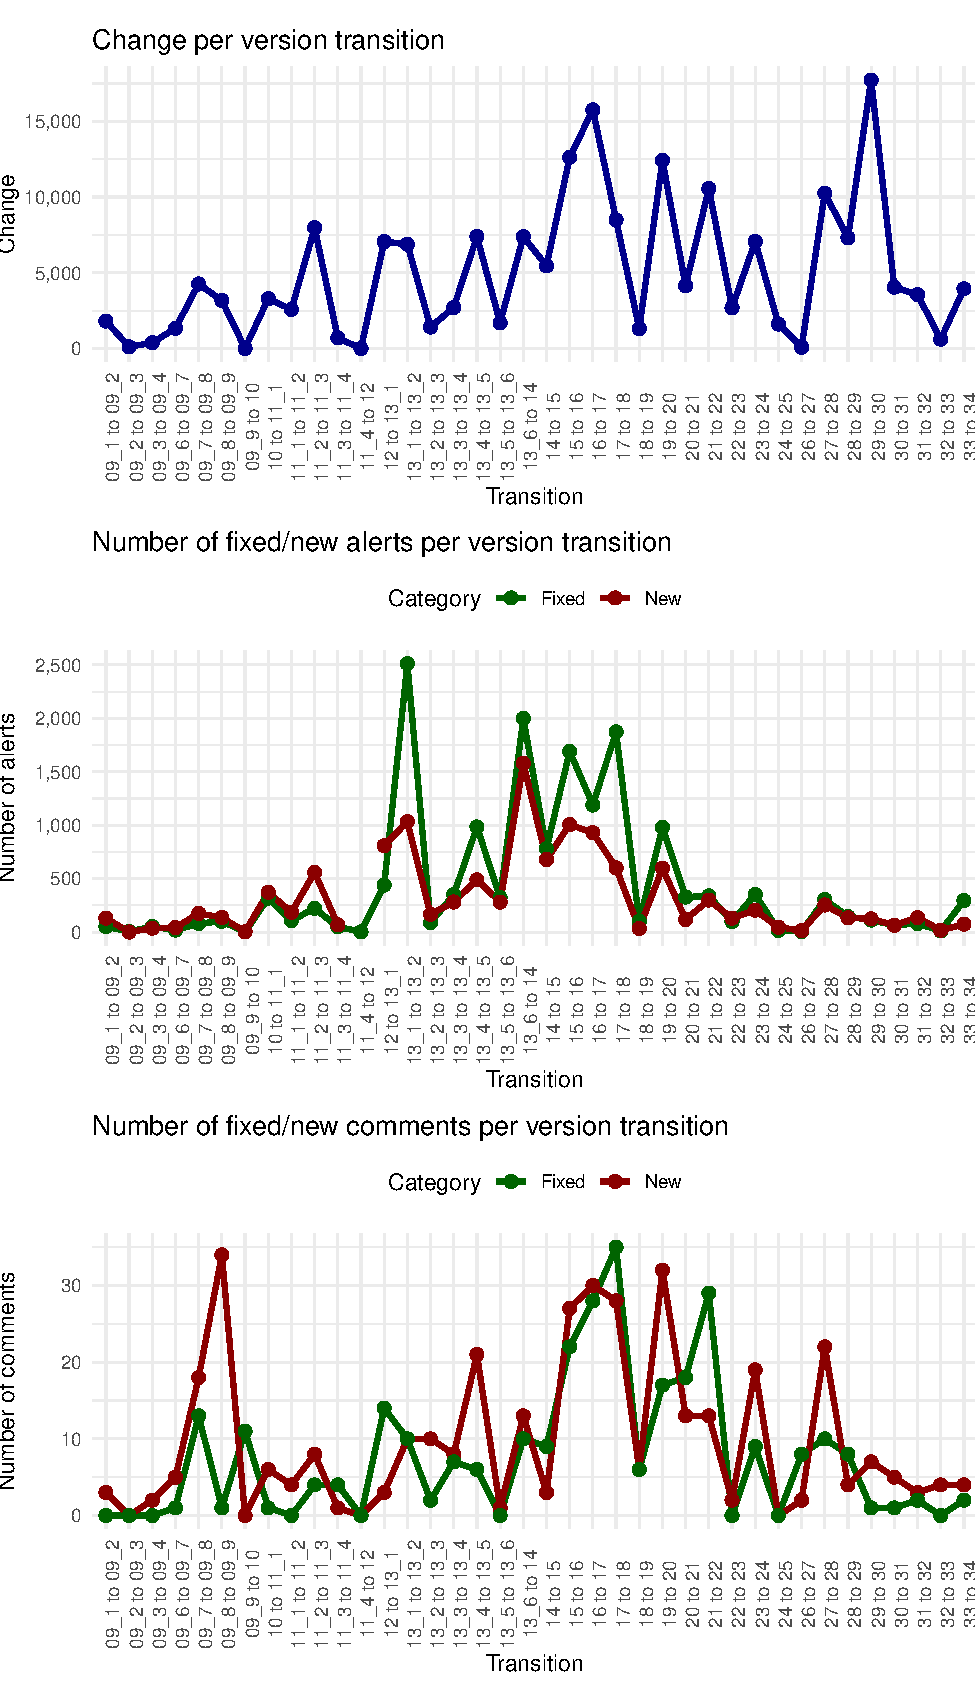
\includegraphics{report_files/figure-latex/unnamed-chunk-26-1.pdf}
\caption{\label{timeseries}Changes, alerts and comments}
\end{figure}

\normalsize

\newpage

We try to measure if there is a correlation between the amount of new
alerts and the amount of new comments.

Figure \ref{scatter_prop} shows the relation between the proportion of
new alerts and the proportion of new comments:

\[PropNewAlerts = \frac{NewAlerts}{NewAlerts + OldAlerts}\]

\[PropNewComments = \frac{NewComments}{NewComments + OldComments}\]

We can see that there is a positive correlation.

\small

\begin{figure}
\centering
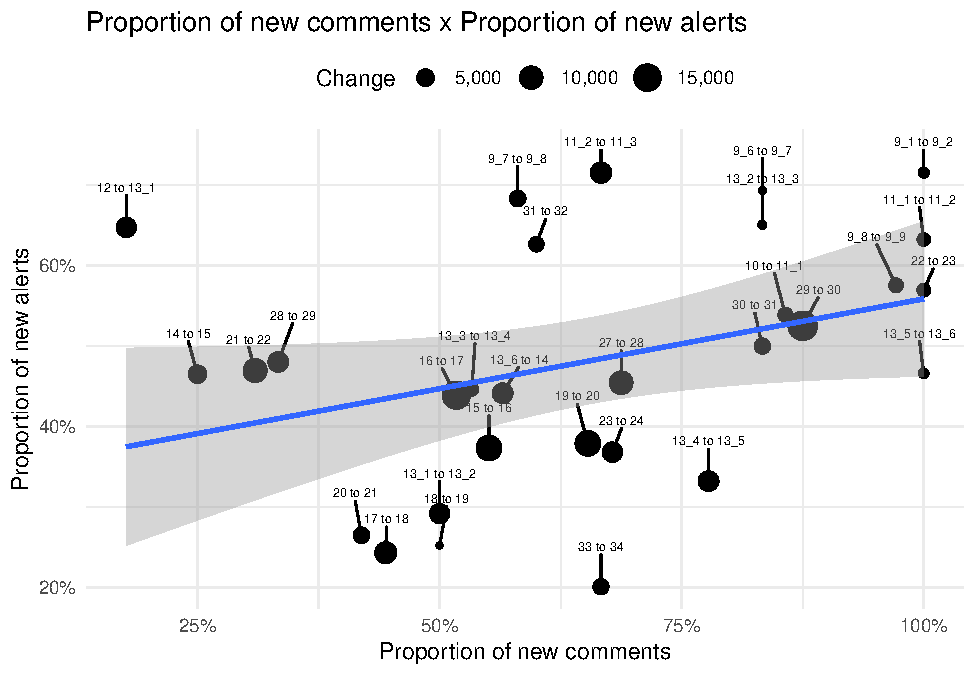
\includegraphics{report_files/figure-latex/unnamed-chunk-27-1.pdf}
\caption{\label{scatter_prop}Proportion of new alerts x Proportion of
new comments}
\end{figure}

\normalsize

In Figure \ref{scatter_diff} we correlate two metrics based on the
difference between the number of alerts and comments normalized by the
amount of change:

\[DiffNewAlerts = \frac{NewAlerts - OldAlerts}{Change}\]

\[DiffNewComments = \frac{NewComments - OldComments}{Change}\]

Where Change is calculated as in Equation \ref{eq_change}.

We can see that there is a positive correlation too.

\small

\begin{figure}
\centering
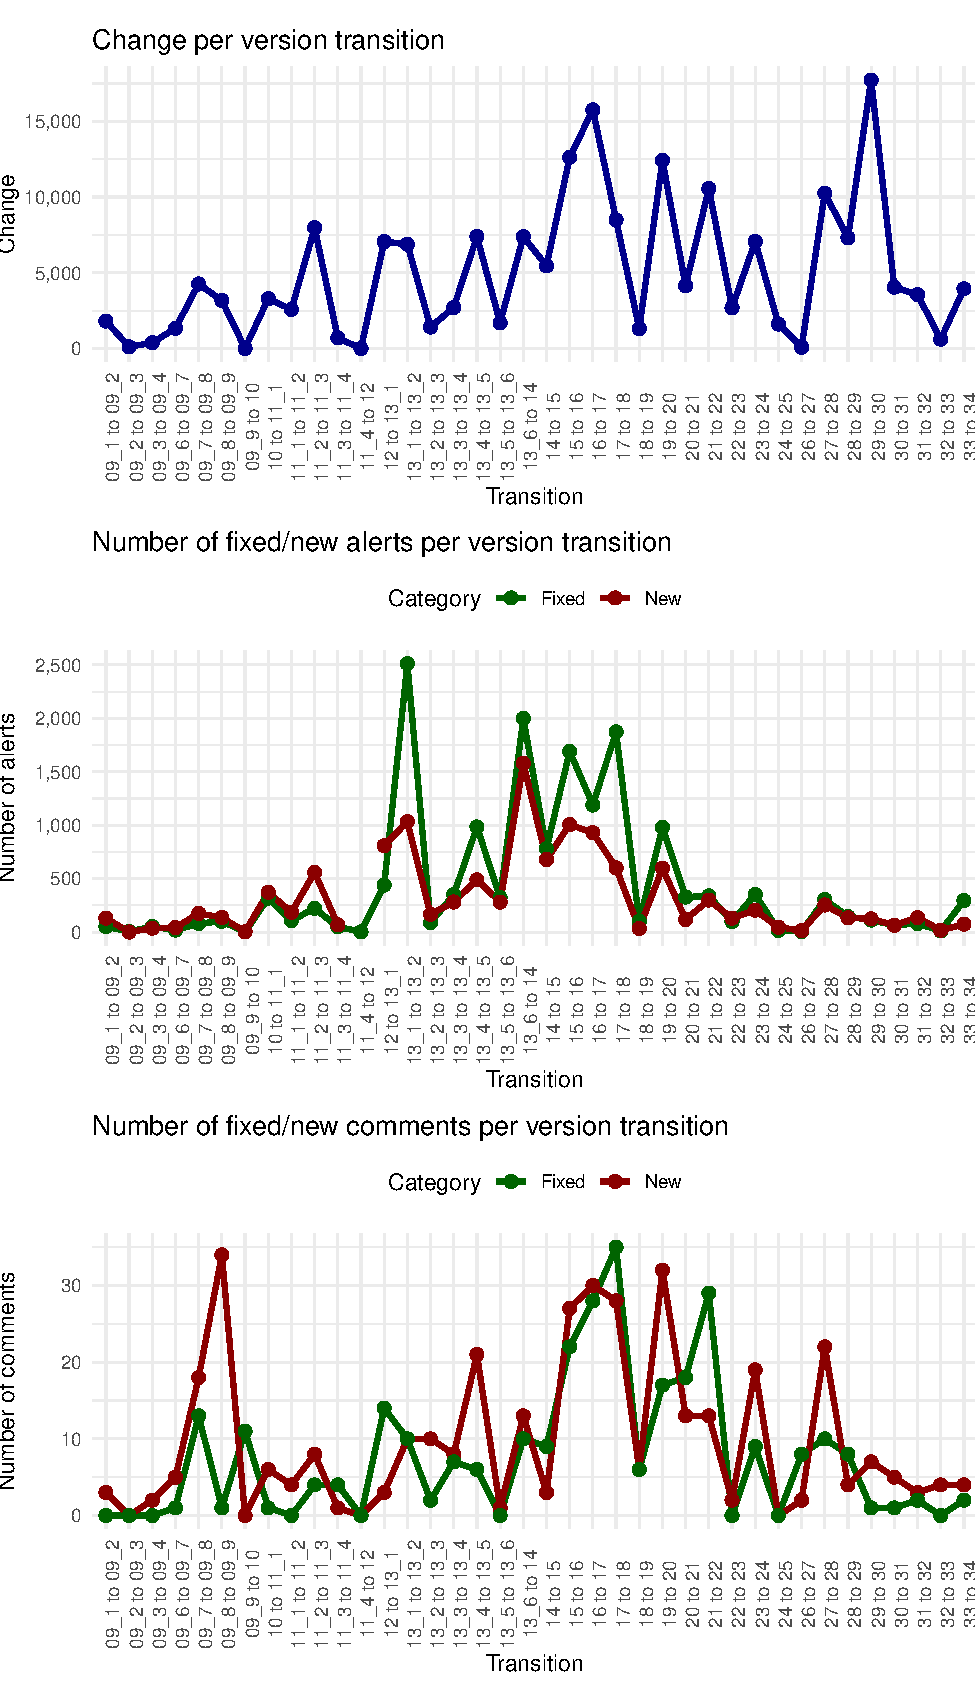
\includegraphics{report_files/figure-latex/unnamed-chunk-28-1.pdf}
\caption{\label{scatter_diff}Proportion of new alerts x Proportion of
new comments}
\end{figure}

\normalsize

It´s necessary to verify if the positive correlation that we found is
statistically significant. Table \ref{tab_reg} shows the results of
these regressions. In the form:

\[ NewAlertsProportion = \alpha + \beta NewCommentsProportions \]

and

\[ AlertsNormalizedDifferences = \alpha + \beta AlertsNormalizedDifferences \]

As we can see by the P-Value of the betas, we cannot reject the null
hypothesis in which there is no relation between comments and alerts.

\small

\begin{table}

\caption{\label{tab:unnamed-chunk-29}\label{tab_reg} Regression: alerts on comments}
\centering
\begin{tabular}[t]{l|l|l|l|l|l|l}
\hline
\multicolumn{1}{c|}{ } & \multicolumn{3}{c|}{Alerts Norm. Differences} & \multicolumn{3}{c}{New Alerts Proportions} \\
\cline{2-4} \cline{5-7}
Characteristic & Beta & 95\% CI & p-value & Beta & 95\% CI & p-value\\
\hline
(Intercept) & 0.34 & 0.17, 0.50 & <0.001 & -0.02 & -0.04, 0.00 & 0.045\\
\hline
New Comments Proportion & 0.22 & -0.01, 0.46 & 0.058 &  &  & \\
\hline
Comments Norm. Difference &  &  &  & 6.5 & -2.6, 16 & 0.16\\
\hline
\multicolumn{7}{l}{\textsuperscript{1} CI = Confidence Interval, CI = Confidence Interval}\\
\end{tabular}
\end{table}

\normalsize

In order to be able to reject the null hypothesis and accept that there
is a correlation between comments and alerts, we must run the same
procedures for more versions of the project and for more projects. We
can refine the way we select the comments, too. There are papers that
use more sofisticated schemes to identify SATD comments. These can be
our next steps.

\section{References}

\hypertarget{refs}{}
\leavevmode\hypertarget{ref-Potdar2014}{}%
Potdar, Aniket, and Emad Shihab. 2014. ``An exploratory study on
self-admitted technical debt.'' \emph{Proceedings - 30th International
Conference on Software Maintenance and Evolution, ICSME 2014}, 91--100.
\url{https://doi.org/10.1109/ICSME.2014.31}.

\leavevmode\hypertarget{ref-Sierra2019}{}%
Sierra, Giancarlo, Emad Shihab, and Yasutaka Kamei. 2019. ``A survey of
self-admitted technical debt.'' Elsevier Inc.
\url{https://doi.org/10.1016/j.jss.2019.02.056}.

\leavevmode\hypertarget{ref-Wehaibi2016}{}%
Wehaibi, Sultan. 2016. ``Satd-Patterns.''
\url{https://github.com/xsultan/satd-patterns}.

\end{document}
